    Très souvent, la résolution d'un problème requiert la présence d'un cadre théorique dans lequel ce problème puisse être formalisé, construit à
    partir d'une compréhension de l'énoncé et du contexte du problème. Ce cadre, plus abstrait, permet alors de résoudre le problème en passant par
    diverses méthodes et manipulations mathématiques, ce que l'on appellerait généralement \emph{calcul} (calcul de nombres, de vecteurs, d'objets
    plus abstraits, \dots).\medskip
    
    La formalisation de ces différentes étapes est étudiée par la \emph{théorie des automates}. Assez récente, elle émerge comme une branche
    indépendante de l'informatique théorique dans la deuxième moitié du \textsc{XX}\ieme~siècle, notamment en 1956 avec la publication des
    \emph{Automata Studies}, compilation des travaux de Claude \textsc{Shannon}, John \textsc{von Neumann}, Edward \textsc{Moore}, Stephen
    \textsc{Kleene}, et autres pionniers de la discipline.\medskip
    
    Le principe de la théorie des automates est de convertir un \guill{problème} en un \emph{langage formel} (le cadre théorique), dans lequel
    l'analyse de certains éléments (le calcul) peut conduire à la résolution du problème. Un \emph{automate} est un objet mathématique abstrait,
    sans existence physique, qui permet de travailler dans ce contexte (\ie d'effectuer les \guill{calculs}).  Ses applications sont nombreuses,
    que ce soit en intelligence artificielle, pour le traitement de texte, en biologie, ou toujours en informatique (les automates sont à la base
    de la théorie de la complexité).Dans ce chapitre, on s'intéressera aux langages formels ainsi qu'aux automates finis, afin de présenter
    plusieurs résultats classiques importants de la théorie des automates.\bigskip
    
    \chaptertoc
    
    \section{Langages réguliers}
    
    \subsection{Alphabets, mots et langages}
    
    \subsubsection{Introduction}
    
    La première composante essentielle à un langage est son alphabet. On a une compréhension assez intuitive de ce concept, ne serait-ce qu'en
    pensant à l'alphabet latin, l'alphabet grec, l'alphabet cyrillique, \etc\!\!. On voit donc un \emph{alphabet} comme un \emph{ensemble} de différents \emph{symboles}, qu'on appelle aussi souvent \emph{lettres}. En
    informatique, on reprend cette notion, en la définissant ainsi :
        
    \begin{definition}{Alphabet, lettres}{}
        On appelle \hg{alphabet} un \hg{ensemble non vide et fini}. On appelle \hg{lettres} ou \hg{symboles} les éléments de cet ensemble.
    \end{definition}
    %
    \begin{notation}
        On désignera usuellement par \hg{$\Sigma$ un alphabet}, et par \hg{$a, b, c, \dots$ les lettres} de $\Sigma$.
    \end{notation}
    
    On donne ci-dessous quelques exemples d'alphabets utilisés en informatique :
    
    \begin{example}{}{}
        \begin{enumerate}
            \itt On a \hg{$\Sigma = \ens{0, 1}$} l'\emph{alphabet} des \hg{nombres en binaire}.
            
            \itt On a $\hg{\Sigma = \ens{a, b, c, \dots, z}}$ l'\emph{alphabet} \hg{latin} (ici constitué des \textit{lettres} minuscules non
            accentuées).
            
            \itt L'\hg{ADN} est constitué de quatre nucléotides (Adénine, Thymine, Cytosine et Guanine), on l'étudie en biologie à l'aide de
            l'\emph{alphabet} $\hg{\Sigma = \ens{A, T, C, G}}$.
            
            \itt On a l'\emph{alphabet} des \hg{caractères \texttt{Unicode}}.
            
            \itt On utilise couramment d'autres \emph{alphabets} de \hg{symboles}, par exemple
            $\hg{\ens{\clubsuit,\diamondsuit,\spadesuit,\heartsuit}}$, $\hg{\ens{+, -, \times, \cdot, \div, \dots}}$ ou
            $\hg{\ens{\rightarrow,\leftarrow,\uparrow,\downarrow}}$
        \end{enumerate}
    \end{example}
    
    Une fois les notions d'alphabet et de lettre introduites, on peut considérer la notion de \emph{mot}, qu'on peut voir comme un $n$-uplet
    (ou comme une suite finie) de lettres d'un alphabet :
    
    \begin{definition}{Mot, longueur}{}
        Soient \hg{$\Sigma$} un \hg{alphabet} et \hg{$n \in \bdN$} un \hg{entier naturel}.
        %
        \begin{enumerate}
            \itast On appelle \hg{mot} (sur $\Sigma$) un \hg{$n$-uplet $u \in \Sigma^n$}.
            
            \itast On appelle \hg{longueur} du mot \hg{$u \in \Sigma^n$} l'\hg{entier $n$}.
            
            \itast On appelle \hg{mot vide} l'unique mot \hg{$\emptyset \in \Sigma^0$} de \hg{longueur nulle}.
        \end{enumerate}
    \end{definition}
    %
    \begin{notation}
        \begin{enumerate}
            \itt On désigne généralement un \hg{mot} par \hg{$u$}, \hg{$v$}, \hg{$w$}, \hg{$x$}, \hg{$y$} ou \hg{$z$}.
            
            \itt On peut représenter le mot \hg{$u = \p{a_1, a_2, \dots, a_n} \in \Sigma^n$} à l'aide ses lettres, selon 
            \hg{$u = a_1a_2\cdots a_n \in \Sigma^\star$}. 
            
            \itt Lorsqu'un \hg{mot} n'est formé \hg{que d'une lettre}, on \hg{identifiera les deux}.
            
            \itt L'\hg{ensemble des mots} sur $\Sigma$ est également noté \hg{$\Sigma^\star$}.
            
            \itt La \hg{longueur du mot $u \in \Sigma^\star$} est notée \hg{$\mod{u}$}.
            
            \itt Le \hg{mot vide} est généralement désigné par \hg{$\epsilon$}.
        \end{enumerate}
    \end{notation}
    
    On donne donc ci-dessous quelques exemples :
    
    \begin{example}{}{}
        \begin{enumerate}
            \itt Considérons l'\hg{alphabet $\Sigma = \ens{a, b, c}$}. On a les mots $\hg{abbca}$ et $\hg{cca}$ de longueur 
            $\hg{\mod{abbca} = 5}$ et $\hg{\mod{cca} = 3}$.
            
            \itt Toujours dans $\hg{\Sigma = \ens{a, b, c}}$, on a l'\hg{ensemble des mots} de longueur inférieure ou égale à $2$ suivant
            %
            \[ \hg{\ens{u \in \Sigma^\star \vphantom{\dfrac{-}{-}}\enstq \mod{u} \leq 2} = \ens{\epsilon, a, b, c, aa, ab, ac, ba, bb, bc, ca, cb,
            cc}} \]
            
            \itt Considérons un microprocesseur de \texttt{64 bits}. On a l'\hg{alphabet $\Sigma = \ens{0, 1}$}.
            
            L'ensemble des \hg{valeurs possibles pour un registre de calcul} est \hg{$\ens{\vphantom{\dfrac{}{}}u \in \Sigma^\star \enstq \mod{u} =
            64}$}. 
        \end{enumerate}
    \end{example}
    
    \textsf{(HPP)} Il peut s'avérer très pratique d'ordonner l'alphabet $\Sigma$, puisque celui-ci est par définition non vide et fini.
    
    \begin{notation}
         On désigne le \hg{nombre d'occurrences d'une lettre $b \in \Sigma$ dans le mot $u = a_1a_2\cdots a_n \in \Sigma^\star$} par $\mod{u}_b$
         %
         \[ \hg{\mod{u}_b = \Card \ens{i \in \iint{1, n} \enstq a_i = b}} \]
    \end{notation}
    
    Lorsque c'est le cas, on peut utiliser le nombre d'occurrences de chaque lettre pour définir la \emph{fonction de \textsc{Parikh}} :
    
    \begin{definition}{Fonction et vecteur de Parikh (HPP)}{}
        Soient \hg{$\Sigma$} un \hg{alphabet} et \hg{$n \in \bdN^\star$} un \hg{entier naturel}, \emph{tel que} \hg{$\Sigma =
        \ens{\sigma_1, \sigma_2, \dots, \sigma_n}$}. 
        %
        \begin{enumerate}
            \itast On appelle \hg{fonction de \textsc{Parikh}} la fonction $\hg{\psi : \begin{array}[t]{ccc}
                \Sigma^\star &\to& \bdN^n  \\
                u &\mapsto& \p{\mod{u}_{\sigma_1}, \mod{u}_{\sigma_2}, \dots, \mod{u}_{\sigma_n}} 
            \end{array}}$.
            
            \itast Pour le \hg{mot $u \in \Sigma^\star$}, on appelle \hg{vecteur de \textsc{Parikh} du mot $u$} le \hg{$n$-uplet $\psi\p{u}$}.
        \end{enumerate}
    \end{definition}
    
    \subsubsection{Concaténation}
    
    On peut dès lors commencer à donner une structure aux notions précédemment définies. Une première opération usuelle est le fait de
    \guill{regrouper} deux mots, \ie la \emph{concaténation} :
    
    \begin{definition}{Concaténation}{}
        Soient \hg{$\Sigma$} un \hg{alphabet}, \hg{$\p{n, m} \in \bdN^2$} deux \hg{entiers}, \hg{$u = a_1\dots a_n \in \Sigma^\star$} un \hg{mot de
        longueur $n$} et \hg{$v = b_1\dots b_n \in \Sigma^\star$} un \hg{mot de longueur $m$}. On appelle \hg{concaténation de $u$ et $v$} le
        \hg{mot $w = a_1\dots a_nb_1 \dots b_n$ de longueur $n + m$}. 
    \end{definition}{}{}
    
    \begin{notation}
        La \hg{concaténation de $u$ et $v$} est généralement notée multiplicativement avec \hg{$u \cdot v$} ou \hg{$uv$}.
    \end{notation}
    
    Immédiatement, il vient :
    %
    \begin{property}{Monoïde $\p{\Sigma^\star, \cdot}$}{}
        Soit \hg{$\Sigma$} un \hg{alphabet}. La \hg{concaténation $\cdot$} est une \hg{loi de composition interne}, \hg{associative} et \hg{de
        neutre $\epsilon$ sur $\Sigma^\star$}.
    \end{property}
    %
    \begin{nproof}
        Soit $\Sigma$ un alphabet, $\p{n, m, p} \in \bdN^3$ trois entiers, et $u = a_1\cdots a_n \in \Sigma^\star$, $v = b_1\cdots b_m \in
        \Sigma^\star$, $w = c_1\cdots c_p \in \Sigma^\star$ trois mots sur $\Sigma$.
        %
        \begin{enumerate}
            \itt $uv \in \Sigma^\star$ est un mot, donc la concaténation $\cdot$ est une loi de composition interne de $\Sigma^\star$.
            
            \itt $u\epsilon = a_1\cdots a_n = \epsilon u = u$, donc $\epsilon$ est un élément neutre de la concaténation $\cdot$.
            
            \itt On a
            %
            \[ \p{uv}w = \p{a_1\cdots a_nb_1\cdots b_m}c_1 \cdots b_p = a_1\cdots a_nb_1\cdots b_mc_1\cdots b_p = a_1 \cdots a_n\p{b_1 \cdots
            b_mc_1 \cdots b_p} = u\p{vw}\]
        \end{enumerate}
        %
        \qquad\quad Donc la concaténation $\cdot$ est associative.
    \end{nproof}
    
    \textsf{(HPP)} En d'autres termes, lorsqu'on muni $\Sigma^\star$ de la concaténation $\cdot$, on obtient le \emph{monoïde non
    commutatif $\p{\Sigma^\star, \cdot}$ de neutre $\epsilon$}. On remarquera également que la longueur $\mod{\cdot} : \begin{array}[t]{ccc}
        \Sigma^\star &\to& \bdN  \\
        u &\mapsto& \mod{u}
    \end{array}$ est un morphisme de monoïde de $\p{\Sigma^\star, \cdot}$ dans $\p{\bdN, +}$. En effet on a $\mod{\epsilon} = 0$ et pour tout
    $\p{u, v} \in \p{\Sigma^\star}^2$, on a $\mod{u \cdot v} = \mod{u} + \mod{v}$.\medskip
    
    On peut également considérer les itérés $n$-ièmes d'un mot par la concaténation. Pour rappel, puisqu'on l'a noté multiplicativement, on devrait
    avoir
    %
    \begin{enumerate}
        \itt $u^0 = \epsilon$
        
        \itt pour tout entier $k \in \bdN$, $u^{k+1} = u \cdot u^k$
    \end{enumerate}
    %
    On définit donc la notion de \emph{puissance d'un mot} :
    
    \begin{definition}{Puissance}{}
        Soient \hg{$\Sigma$} un \hg{alphabet}, \hg{$n \in \bdN$} un \hg{entier} et \hg{$u \in \Sigma^\star$} un \hg{mot} sur $\Sigma$. On appelle
        \hg{puissance $n$-ième de $u$} le \hg{$n$-ième itéré} de \hg{$u$} par la \hg{concaténation}. On pourra parler de \hg{puissance carré} pour
        la \hg{puissance $2$-ième}, de \hg{puissance cubique} pour la \hg{puissance $3$-ième}, \etc\!\!.
    \end{definition}
    %
    \begin{notation}
        La \hg{puissance $n$-ième de $u$} sera généralement notée \hg{$u^n = \underbrace{u \cdot u \cdot \dots \cdot u}_{n \ \text{fois}}$}
        (notation mulitplicative de l'itéré).
    \end{notation}
    
    On donne ci-dessous quelques exemples des concepts précédemment introduits :
    
    \begin{example}{}{}
        On considère l'\hg{alphabet $\Sigma = \ens{a, b, c}$}, le \hg{mot $u = ab \in \Sigma^\star$} et le \hg{mot $v = cab \in \Sigma^\star$}. On
        a :
        %
        \begin{enumerate}
            \itt \hg{$uv = u \cdot v = abcab \in \Sigma^\star$} (concaténation de $u$ et $v$).
            
            \itt \hg{$v^2 = v \cdot v = cabcab \in \Sigma^\star$} (puissance carré de $v$).
            
            \itt \hg{$vu^2 = v \cdot u^2 = v \cdot u \cdot u = cababab \in \Sigma^\star$} (concaténation de $v$ et de la puissance carré de $u$).
            
            \itt \hg{$c\p{ab}^3 = c \cdot \p{ab}^3 = cababab \in \Sigma^\star$} (concaténation du mot/lettre $c$ et de la puissance cubique du mot
            $ab$).
            
            \itt \hg{$a^4b^2c^2 = aaaaabbcc \in \Sigma^\star$} (concaténation de puissances des mots/lettres $a$, $b$ et $c$).
        \end{enumerate}
    \end{example}
    
    Inversement, on peut voir tout mot comme la concaténation de plusieurs \guill{sous-mots} (cette appellation désigne en fait un concept plus
    large, qu'on présentera juste après). Même dans le cas d'un simple mot d'une lettre, on peut le voir comme la concaténation de lui-même avec le
    mot vide $\epsilon$. En effet, on peut remarquer
    %
    \[ \forall u \in \Sigma^\star,\qquad u = \epsilon\cdot u = u \cdot \epsilon \]
    %
    Ainsi on définit :
    
    \begin{definition}{Préfixe, suffixe}{}
        Soient \hg{$\Sigma$} un \hg{alphabet} et \hg{$\p{u, v, w} \in \p{\Sigma^\star}^3$} trois \hg{mots} sur $\Sigma$ tels que \hg{$u = v \cdot w
        = uv$}.
        %
        \begin{enumerate}
            \itast On dit que \hg{$v$} est un \hg{préfixe de $u$}. On dit que c'est un \hg{préfixe propre de $u$} lorsque \hg{$v \neq \epsilon$} et
            \hg{$v \neq u$}.
            \itast On dit que \hg{$w$} est un \hg{suffixe de $u$}. On dit que c'est un \hg{suffixe propre de $u$} lorsque \hg{$w \neq \epsilon$} et
            \hg{$w \neq u$}.
        \end{enumerate}
    \end{definition}
    
    \begin{notation}
        Pour un \hg{mot $u \in \Sigma^\star$}, on note \hg{$\Pref\p{u}$} l'\hg{ensemble de ses préfixes} et \hg{$\Suff\p{u}$} l'\hg{ensemble de ses suffixes}.
    \end{notation}
    
    On définit également la notion de \emph{facteur} :
    
    \begin{definition}{Facteur}{}
        Soient \hg{$\Sigma$} un \hg{alphabet} et \hg{$\p{u, v} \in \p{\Sigma^\star}^3$} deux \hg{mots} sur $\Sigma$. On dit que \hg{$v$ est un facteur de $u$} lorsque :
        %
        \[ \hg{\exists \p{w_p, w_s} \in \p{\Sigma^\star}^2,\qquad u = w_p \cdot v \cdot w_s = w_pvw_s}\]
        %
        On dit que c'est un \hg{facteur propre de $u$} lorsque \hg{$v \neq \epsilon$} et \hg{$v \neq u$}.
    \end{definition}
    
    \begin{notation}
        Pour un \hg{mot $u \in \Sigma^\star$}, on note \hg{$\Fact\p{u}$} l'\hg{ensemble de ses facteurs}.
    \end{notation}
    
    On remarquera que la notion de facteur généralise celle de préfixe et de suffixe, et particulièrement que
    %
    \[\forall u \in \Sigma^\star,\qquad \Pref\p{u} \subset \Fact\p{u} \quad\et\quad \Suff\p{u} \subset \Fact\p{u} \]
    %
    c'est-à-dire que tout préfixe et tout suffixe d'un mot est un facteur de ce mot.
    
    \begin{example}{}{}
        On considère l'\hg{alphabet $\Sigma = \ens{a, b, c}$}, et le mot \hg{$u = abbc \in \Sigma^\star$}. On a :
        %
        \begin{enumerate}
            \itt Les \hg{préfixes} de $u$ sont \hg{$\Pref\p{u} = \ens{\epsilon, a, ab, abb, abbc}$}.
            
            \itt Les \hg{suffixes} de $u$ sont \hg{$\Suff\p{u} = \ens{\epsilon, c, bc, bbc, abbc}$}.
            
            \itt Les \hg{facteurs} de $u$ sont \hg{$\Suff\p{u} = \ens{\epsilon, a, b, c, ab, bb, bc, abb, bbc, abbc}$}.
        \end{enumerate}
    \end{example}
    
    On peut 
    

    
    \begin{definition}{Sous-mot}{}
        Soit $w=a_1 \dots a_n$ un mot sur $\sigma$.
        Un \hg{sous-mot} est un mot de la forme $a_{i_1} \dots a_{i_k}$ avec $1 \leq i_1 < \dots < i_k \leq n$
        
    \end{definition}
    
    \begin{warning}{}{}
        Ne pas confondre "facteur" et "sous-mot".
        \begin{enumerate}
            \itt bca est un facteur de w.
        \end{enumerate}
    \end{warning}
    
    \begin{example}{}{}
        $w=abcabc$
        \begin{enumerate}
            \itt $bca$ a est un sous mot de $w$
            \itt $abab$ est un sous mot de $w$
            \itt $cac$ est un sous mot de $w$
            
            
        \end{enumerate}
        
        On remarque que les relations "être préfixe, suffixe, facteur, sous-mot" sont des \hg{relations bien fondées} sur $\sigma^\star$.
        
    \end{example}
    \begin{definition}{mot miroir}{}
        \begin{enumerate}
            \itt on appelle mot miroir de w et note $w^R$
        le mot $w^r =  a_1 \dots a_n$
            \itt un palindrome est un mot qu'on peut lire dans les deux sens tel que $w=w^R$
            
            
            
        \end{enumerate}
        
    \end{definition}
    
    \begin{definition}{Langage}{}
        Un langage $L$ sur un alphabet $\Sigma$ et un sous ensemble $\Sigma^*$ 
    \end{definition}
    
    \begin{example}{}{}
        On prend $\Sigma = \ens{a, b, c}$.
        %
        \begin{enumerate}
            \itt $L_1 = \ens{abc, bca, acb}$ est un langage fini.
            
            \itt $L_2 = \ens{ab^nc \enstq n \in \bdN}$ est le langage infini des mots commençant par $a$; suivi d'une suite (de taille arbitraire) de $b$, et finissant par $c$.
            
            \itt $L_3 = \ens{a^n \enstq n \in \bdP}$
        \end{enumerate}
    \end{example}
    
    \begin{notation}
        On note $\overline{L}$ le complémentaire de L :
        $\overline{L} = \Sigma^* \backslash L$
    \end{notation}
    
    \begin{definition}{Concaténation de deux langages}{}
        Soit $L_1 et L_2$ des langages sur $\Sigma$.
        Le langage \hg{concaténation}  de $L_1$ et $L_2$, noté $L_1 L_2$, est défini par :
        $L_1 L_2 = \ens{\omega \enstq \exists u \in L_1, \exists v \in L_2, \omega = uv}$
    \end{definition}
    
    \begin{example}{}{}
        $L_1 = \ens{aa, ab, bc} ; L_2 = \ens{\epsilon, a, abc}$
        $L_1 L_2 = \ens{aa, ab, bc, aaa, aba, bca, aaabc, ababc, bcabc}$
    \end{example}
    
    \begin{definition}{Puissance d'un language }
        Soit $L \subset \Sigma^*$, Soit $n\in \bcN$  
        
        
        Le langages $L^n$ est definit par récurrence sur $n$
        \begin{enumerate}{}{}
            
            \itt $L^0 = \ens{ \varepsilon}$
            
            \itt %lol itt comme un jour d'itt 
                $L^n+1 = L * L^n $ pour $n \geq 0$ 
                
        \end{enumerate}{}
        
    \end{definition}
    
    \begin{warning}{}{}
        \begin{enumerate}
            \itast Ne pas confondre $\emptyset$ et $\ens{\epsilon}$
            
            \itast Ne pas confondre $L^n$ et $\ens{u^n \enstq u \in L}$
        \end{enumerate}
    \end{warning}
    
    \begin{definition}{Étoile de Keeme}{}
        Soit \hg{$L \subset \Sigma^\star$}. On appelle \hg{étoile de \textsc{Kleene} de $L$} le langage \hg{$\displaystyle \bigcup U_{n \in \bdN} L^n$}.
    \end{definition}
    
    \begin{notation}
        L'\hg{étoile de \textsc{Kleene} de $L$} est généralement notée \hg{$L^\star$}.
    \end{notation}
    
    On remarque que
    \begin{enumerate}
        \itt c'est de la que vient la notation $\Sigma^\star$
        \itt On note parfois $L^+ = \bigcup_{n > 0} L^n$
    \end{enumerate}
    
    \begin{definition}{langage miroir}{}
        Soit $L \subset \Sigma^\star$. On appelle langage mirroir de L le langage $L^r$ défini par $L^r = \ens{\omega^r \enstq \omega \in L}$
        
    \end{definition}
    
    \subsection{Langage réguliers, expression régulières}
    
    \begin{definition}{Langage réguliers}{} 
        Soit $\Sigma$ un alphabet. L'ensemble des langages réguliers sur $\Sigma$ (ou langages rationnels sur $\Sigma$) est défini inductivement par: 
        \begin{enumerate}
            \itast $\emptyset$ est un langage régulier
            
            \itast  Pour tout $a \in \Sigma$, $\ens{a}$ est régulirer ;
            
            \itast si $A$ et $B$ sont des langages réguliers, alors $A \cup B$, $AB$ et $A^\star$ sont réguliers.
            
        \end{enumerate}
    \end{definition}
    %
    \begin{notation}
        On note $\Reg_\Sigma$ l'ensemble des langages réguliers sur $\Sigma$.
    \end{notation}
    
    Parfois, on inclut dans la définition précédente que $\ens{\epsilon}$ est régulier. Ceci est en fait redondant car $\ens{\epsilon} = \emptyset^\star$
    
    \begin{definition}{Expression régulière}{}
        
        Une expression régulière sur un alphabet $\Sigma$ ou expression rationnelle est définie inductivement 
        %
        \begin{enumerate}
            \itast $\emptyset$ et $\epsilon$ sont*µ des expressions régulières.
            
            \itast pour tout $e \in \Sigma$, $e$ est une expression régulière.
            
            \itt si $r_1 et r_2$ sont deux expression réguliere 
                \begin{enumerate}
                    \itt $r_1 | r_2$ est une expression réguliere 
                    
                    \itt $r_1, r_2$ est une expression régulière
                    
                    \itt $r_1^* $ est une expression régulière
                \end{enumerate}
        \end{enumerate}
    \end{definition}
    
    On notera que les règles de priorité sont ${}^\star > \cdot > \vert$.
    
    
    \begin{definition}{Langage d'une expression reguliere}{}
        Soit r une expression reguliere sur $\Sigma$
        
        le langage de l'equation r, noté $\bsL(r)$, est defini par induction structurelle sur r≠
        
        
        \begin{enumerate}
            \itt $\bsL\p{\emptyset} = \ens{\emptyset}$
            \itt $\bsL\p{\epsilon} = \ens{\epsilon}$
            \itt $\forall a \in \Sigma, \bsL\p{a} = \ens{a}$
            \itt $\bsL\p{r_1 \enstq r_2} = \bsL \p{r_1} \cup \bsL \p{r_2}$
            \itt $\bsL\p{r_1 r~……∞,_2} = \bsL \p{r_1} \bsL \p{r_2}$
            \itt $\bsL\p{r^\star} = \bsL \p{r}^\star$ 
        \end{enumerate}
    \end{definition}{}
    
    \begin{example}{}{}
        \begin{enumerate}
            \itt $mpi^\star : \ens{mpi \dots i}$
            \itt $\p{mpi}^\star : \ens{mpimpi \dots mpi}$
            
            \itt L'ensemble des nombres en base 2 sans zéro non significatif est reconnu par
            $0 \vert 1 \p{0 \vert 1}^\star$
            
            \itt $0^\star 1 0^\star 1 0^\star 1 0^\star$ décrit le langage des mots sur $\Sigma = \ens{0, 1}$ contenant exactement trois 1.
        
            \itt $\p{a \vert b \vert c \vert \dots \vert z \vert .\vert-}^\star @ \p{a \vert \dots \vert z \vert -}.\p{com \vert fr \vert \dots}$
            est l'ensemble des adresses mails syntaxiquement correctes.
        \end{enumerate}
    \end{example}
    
    \begin{enumerate}
        \itt En anglais, le terme \textit{regular expression} est souvent abrégé en \textit{regex}.
        
        \itt sous \textit{Linux}, l'outil \texttt{grep} permet de rechercher un motif dans des fichiers a l'aide d'expression régulières :
        %
        \[ \text{\sffamily\textbf Globally \textbf regular \textbf expression \textbf print }\]
        
        L'outil \texttt{grep} utilise une syntaxe étendue (\textsf{POSIX}) pour décrire les expressions régulières (\cf TP1).
        
    \end{enumerate}
    
    \section{Automates finis}
    
    Les automates sont des objets calculatoires fondamentaux a l'informatique.
    Il en existe de nombreusses variantes, selon le domaine d'application 
    \begin{enumerate}
        
        \itt automates finis 
        \itt automates à pile 
        \itt automates d'arbre 
        \itt automates àcompteurs 
        \itt automates temporisés 
        
    \end{enumerate}
    
    Voici quelque applications
    
    \begin{enumerate}
        \itt analayse de texte 
        \itt blabla  blabla 
        \itt blablab blabla 
        \itt blablablbla
        
        \itt IA 
        
        \itt ...
        
    \end{enumerate}
    
    \subsection{Automates déterministes}
    
    \begin{definition}{automates fini déterministes complet}{}
        
        Un \hg{automates fini déterministe complet} (ou CDFA) 
        
        est un quintuplet $\bcA$ = $Q,\Sigma, q_0, F, \sigma$
        \begin{enumerate}
            \itt $Q$ est un ensemble fini d'\hg{états}
            \itt $\Sigma est un alphabet$
            \itt $q_0 \in Q$ est l'\hg{état initial}
            \itt $F \subset Q$ est l'ensemble des \hg{états finaux} (\hg{ou acceptants})
            \itt $\sigma :  Q  *  \Sigma -> Q $est une fonction totale, appeler fonction de l'automate.   
        
        \end{enumerate}
    
    \end{definition}
    
    \begin{example}{}{}
        $\bsA_{bin} = \p{\ens{q_0, q_1, q_2, q_\bot}, \ens{0, 1}, q_0, \ens{q_1, q_2}, \delta_{bin}}$
        
        avec $\sigma_{bin} :$
        \begin{enumerate}
            \itt $\p{q_0, 0} \to q_1$
            \itt $\p{q_0, 1} \to q_2$
            \itt $\p{q_1, 0} \to q_\bot$
            \itt $\p{q_1, 1} \to q_\bot$
            \itt $\p{q_2, 0} \to q_2$
            \itt $\p{q_2, 1} \to q_2$
            \itt $\p{q_\bot, 0} \to q_\bot$
            \itt $\p{q_\bot, 1} \to q_\bot$
        \end{enumerate}
    \end{example}
    \begin{notation}
        représentation d'un automates par un graphe
        
        \begin{enumerate}
            \itt chaque état est un sommet du graphe (q)
            
            \itt l'état initiale est indiqué par une flèche entrante: ($--> q_0$)
            
            \itt si $q_f \in F$, il est entouré 2 fois.
            
            \itt si $\delta \p{q_1, a} = q_2$ on a un arc.
            
            
        \end{enumerate}
        
        
    \end{notation}
     
    \begin{example}{}{}
        L'automate $\Atom$ peut être représenté comme suit :
        
        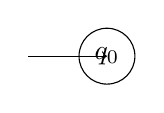
\begin{tikzpicture}
            \draw[->] (0, 0) -- (1, 0);
            
            \node[draw, circle] at (1, 0) {$q_0$} ;
        \end{tikzpicture}
        
    
        
    \end{example}
    \begin{definition}{chemin}{}
        Soit $\bcA = (Q,\Sigma, q_0, F, \delta)$ sur CDFA.
        
        
        Soit $v = a_1 \dots a_n  \in \Sigma^\star$ 
        
        Le chemin est dit \hg{acceptant} si $r_0 = q_0 et r_a \in F$
        On dit que $\bsA$ \hg{reconnaît} (ou \hg{accepte}) le mot $v$ s'il existe un chemin l'acceptant par v dans $\bsA$
        
    \end{definition}
    
    \begin{notation}
        \begin{enumerate}
            \itt On note $r_0\lima{a_1} r1 \lima{a_2} \dots r_{n - 1} \lima{a_n} r_n$ un chemin.
            \itt Si on ne souhaite pas spécifier tout les états intermédiaires on note $r_0 \lima{v} r_n$ lorsqu'il n'y a pas de doute sur $\bsA$.
        \end{enumerate}
    \end{notation}
    
    \begin{example}{}{}
        \begin{enumerate}
            \itt $v = 0 : q_0 \lima{0} q_1 \in F$ donc 0 est accepté par $\bsA_{bin}$.
            \itt $v = 101 : q_0 \lima{1} q_2 \lima{0} q_2 \lima{1} q_2 \in F$ Donc 101 est accepté
            \itt $v = 010 : q_0 \lima{0} q_1 \lima{1} q_\bot \lima{0} q_\bot \notin F$
        \end{enumerate}
    \end{example}
    
    On remarque que si $q \in Q$ est tel que :$\forall a \in \Sigma, \delta \p{q, a} = q$, on dit que $q$ est un état absorbant.
    
    \begin{example}{}{}
        $q_1 et q_2$ sont des états absorbants de $\bsA_{bin}$.
    \end{example}
    
    \begin{definition}{Langage d'un automate}{}
        Soit $\bsA$ un automate. Le langage de $\bsA$, noté $\bsL \p{\bsA}$, est l'ensmeble des mots acceptés par $\bsA$.
    \end{definition}
    
    \begin{example}{}{}
        $\bsL \p{\bsA_{bin}} = 0 \vert 1 \p{0 \vert 1}^\star$
    \end{example}
    
    \begin{definition}{automate déterministe incomplet}{}
        Un automae deterministe incomplet (DFA)
        est un quintuplet $\bcA = (Q,\Sigma, q_0, F, \delta)$ dont - $Q,
        \Sigma, q_0 et F$ sont definis comme pour ∞ les CDFA 
             
             - $\delta :  Q * \Sigma -> Q $ est une fonction partielle 
    \end{definition}
    
    \begin{example}{}{}
        $\bsA_{bin}'$ \newline
        schéma 2 \newline
        $\bsL \p{\bsA_{bin}'} = \bsL \p{\bsA_{bin}}$
    \end{example}
    
    
    On remarque que dans un CFDA $\bcA$, pour tout $v\in \Sigma^*$, il y a un unique chemin associé a $v$ partant de $q_0$ dans $\bcA$
    
    \begin{theorem}{completion}
        Soit $A$ = $\bcA = (Q,\Sigma, q_0, F, \delta)$ un DFA 
        il existe un unique DFA CDFA $A_c$ tel que $\bsL(A_i) = \bsL(A_c) $
        
        what do you do mean  
             
                
        
    \end{theorem}  
    
    \begin{nproof}
        On pose $\bsA_c = \ens{Q_a, \Sigma, q_0, F, \delta}$ où
        \begin{enumerate}
            \itt $Qc = Q_i \cup \ens{q_\bot}$ avec $q_\bot \notin Q_i$
            \itt $\delta_c \times \Sigma \to Q_c$ telle que :
            \begin{enumerate}
                \itt $\p{q, a} \to \delta_i \p{q, a \in dom \p{\delta_i}}$ % dom -> domaine
                \itt $(q, a) \to q_\bot si \p{q, a} \notin dom \p{\delta_i}$
                \itt $\p{q_\bot, a} \to q_\bot \forall a \in \Sigma$
            \end{enumerate}
            
        \end{enumerate}
        $q_\bot$ est appelé état pridr
        
        Montrons que $\forall v \in \Sigma^\star, v \in \bsL \p{\bsA_i} \equiv v \in \bsL \p{1_c}$
        
        $\implies$ : Si $v = q_1 \dots q_n \in \bsL \p{\bsA_i}$, alors $q_0 \lima{v}_{\bsA_i}^\star q_f \in F$. On a alors $q_0 \lima{v}_{\bsA_c}^\star q_f$, et $v$ accepté par $\bsA_c$ car :
        \begin{enumerate}
            \itt $q_0$ est l'état initial de $\bsA_c$
            \itt $F$ est l'ensemble des états finaux de $\bsA_c$
            \itt $\delta_i$ et $\delta_c$ coïncident sur deux $\p{\sigma_i}$
        \end{enumerate}
        
        
        <==
        Par contraposé: Si $v \notin \bsL(A_i) $
        \begin{enumerate}
            \itt il existe un chemin $q_0$ --------> q'. 
        
            puisque $v \not \in \bsL(A_i), q \notin F $
            
            on a donc $q_0 -------> q' \notin F $ donc $v \in \bsL(A_c)$.
            \itt si il existe pas de chemin dans $\bcA_i$ partant $q_0$ pour $v=q_1 \dots q_n$
        
        donc $\exists x \in $ [|0, n-1|] tq $u=a_1 \dots a_k$ possède un tel chemin mais pas $u_(a_k+1)$
        \end{enumerate}
        
        $q_0 = r_0 \lima{a_1} r_1 \lima{a_2} r_2 \dots \lima{a_k} r_k$ et $\p{r_k, a_{k+1}} \notin dom \p{\delta_i}$
        on a donc le chemin
        $q_0 = r_0 \lima{a_1} r_1 \lima{a_2} r_2 \dots \lima{a_k} r_k \lima{a_{k+1}} q_\bot \dots \lima{a_n} q_\bot \notin F$
            
        
        Donc $v \notin \bsL(A_c)$
    \end{nproof}
    
    
    
    \begin{example}{}{}
        $\bcA_bin$ est le completé de $\bcA_bin'$
        par se prossesus 
        
    \end{example}
    
    \begin{definition}{etat accesible}{}
        Soit $\bsA = \ens{Q, \Sigma, q_0, F, \delta}$ un DFA.
        Un état $q \in Q$ est dit \hg{accessible} si $\exists v \in \Sigma^\star$ tel que $q_0 \lima{v}_\bsA^\star q$
    \end{definition}
    
    On remarque que pour trouver l'ensemble des "tats accessibles, il suffit de faire un parcours de graphe en partant de $q_0$.
    
    \begin{definition}{etat coaccessible}{}
        
        Soit $\bsA_c = \ens{Q_a, \Sigma, q_0, F, \delta}$ un DFA.
        
        Un etat $q\in Q$ est dit co-accesible si 
        
        $\exists v \in \Sigma^*$, $\exists q_f \in F $ tq $ q \lima{v *}{\bsA} q_f$
        
    \end{definition}
    
    On remarque que pour trouver l'ensemble des état co-accessible, on peut faire un parcours de graphe en partant des états $q_f \in F $ et on remantant les arcs.
    
    \begin{example}{}{}
        % INSERT schéma 3 HERE
        \text{}\newline
        schéma 3 \newline
        
        \begin{enumerate}
            \itt $q_0$ et $q_1$ sont co-accessibles
            \itt $q_2, q_3, q_4$ ne sont pas co-accessibles
        \end{enumerate}
    \end{example}
    
    
    \begin{definition}{état utile}
        Soit $\bsA = \ens{Q, \Sigma, q_0, F, \delta}$ un automate
        Un état $q \in Q$ est dit utile s'il est a la fois accessible est co-accessible 
        
    \end{definition}
    \begin{definition}{émondé}{}
        Un automate est dis émondé si tous ces état ces état sont utiles 
    \end{definition}
    On remarque que émondé n'implique pas qu'il soit le plus petit possible  
    
    \begin{example}{}{}
        \text{}\newline
        DESSIN de rayan "schéma 3"  
        \newline 
        $\bcA$ et $\bcA'$ sont émondés et $\bcL\p{\bcA} = \ens{a, b}^\star = \bcL\p{A'}$.
    \end{example}
    
    \subsection{Automates non déterministes}
    
    \begin{definition}{Automate fini non déterministe}
        On appelle automate fini non déterministe (NFA) un quintuplet $\bcA = \p{Q, \Sigma, q_0, F, \delta}$ où :
        %
        \begin{enumerate}
            \itast $Q$, $\Sigma$, $q_0$, $F$ sont définis comme pour les DFA ;
            
            \itast $\delta : Q \times \Sigma \to P\p{Q}$ est une fonction partielle appelée \hg{relation de transition}.
        \end{enumerate}
    \end{definition}

    \begin{definition}{Chemin}{}
        Soit $\bsA = \ens{Q, \Sigma, q_0, F, \delta}$ un NFA 
        Soit $v = a_1 \dots a_n \in \Sigma^\star$.
        
        Un chemin dans $\bcA$ pour $v$ est une séquence de $n+1$ états $r_0, r_1, \dots, r_n$ tels que :
        
        \begin{enumerate}
            \itast $\forall i \in \iint{0, n}$, $r_i \in Q$.
            
            \itast $\forall i \in \iint{1, n}, r_i \in \delta\p{r_{i-1}, a_i}$.
        \end{enumerate}
    
    le chemin est dis acceptant si $r_0=q$ et $r_n \in F$.
    Un mot $v$  est accepté par $\bcA$ si $\exists$ un chemin acceptant pour $v$ dans $\bcA$ . 
    
    %???????????????????????
    
    
    \end{definition}
    
    \begin{example}{}{}
        $\bcA_{a3} :$
        %
        \newline
        Dessin 4
        \newline 
        
        \begin{enumerate}
            \item 
            
            
            \itt $abaa \notin \bsL(\bcA_{a3})$
        \end{enumerate}
    \end{example}
    %mdrrrrr y a un stack d'erreur (64)
    
    
    remarque: Pour tester si $v\in \bsL\p{bsA} a$ avec $\bsA$ un NFA, il faut "deviner" le chemin qui va être acceptant : il faut a priori tous les tester jusqu'a ce qu'il y en ai un qui marche. On peut utiliser le backtracking.
    
    \begin{definition}{}{}
        Un automates finis (non déterministe) 
        à transition spontanné ($\varepsilon -$NFA) %NFA comme nouveau pere fondateur 
        est un quintuplet $\bsA = \ens{Q, \Sigma, q_0, F, \delta}$ ou 
        
        \begin{enumerate}
            \itt $Q, \Sigma, q_0, F$ sont définis comme pour les NFA
            \itt $\delta Q x \p{\Sigma \cup \ens{\epsilon}} \to \bsP \p{Q}$ est une fonction partielle
        \end{enumerate}
        
    \end{definition}
    
    On remarque que dans $v_n$ les $\varepsilon$ - NFA,  les transitions de la forme $q \lima{\epsilon} q'$ sont appelées des transitions spontanées (ou $\epsilon$ transition).
    
    
    \begin{definition}{chemin}{}
        Soit $\bsA = \p{Q, \Sigma, q_0, F, \delta} un \epsilon-NFA$ Soit $v \in \Sigma^\star$ Un chemin dans $\bsA$ pour v est une séquence finie $r_0, \dots , r_n$ de $n+1$ états tq :
        
        \begin{enumerate}
            \itt $\exists (a_1, \dots, a_n) \in \p{\Sigma \cup \ens{\epsilon}}^n tq v = a_1 \dots a_n$
            \itt $\forall i \in \iint{0, n}, r_i \in Q$
            \itt $\forall i \in \iint{1, n}, r_i \in \delta \p{r_{i-1}, a_i}$
        \end{enumerate}
            
    \end{definition}
    
    \begin{example}
            \newline
            dessin 5 sur le discord
            \newline
            
            \begin{enumerate}
                \itt $\epsilon \in \bsL \p{\bsA}$
                \itt $ac \in \bsL \p{\bsA}$
                \itt $bbbb \in \bsL \p{\bsA}$
            \end{enumerate}
        $\bsL \p{\bsA} = \p{a \enstq b}^\star b^\star c^\star$
        $ = \p{a \enstq b}^\star c^\star$
    \end{example}{}
    
    \subsection{Déterminisation, suppression des $\varepsilon$-transitions}
    
    Nous avons introduit 3 modèles d'automates: les DFA, les NFA, et les $\epsilon$-NFA. Nous allons maintenant montrer que ces 3 modèles sont équivalents.
    
    %%go pour une preuve qui fais 3 tableaux avec 50 schémas  
    
    
    \begin{definition}
        Soit $\bcA_N = \ens{Q_N, \Sigma, q_0, F_N, \delta_N }$ un NFA
        
        
        On appelle automates des parties de $\bcA_N$, noté $\det(\bcA_n)$
        l'automate déterministe $\bcA_D = \ens{Q_D, \Sigma, \ens{q_0}, F, \delta_D}$ tel que :
        %
        \begin{enumerate}
            \itast $Q_D = P\p{Q_N}$
            
            \itast $F_D = \ens{S \enstq S \subseteq Q_N, S \cap F_N \neq \emptyset }$
            
            \itast $\delta_D : \begin{array}[t]{rcl}
                Q_D \times \Sigma &\to& Q_D  \\
                \p{S, a} &\mapsto& \displaystyle\bigcup_{q \in S} \delta_N\p{q, a} 
            \end{array}$
        \end{enumerate}
        
        
    \end{definition}
    
    \begin{example}{}{}
            %j'ai pris une photo et je l'ai giga compresser 
        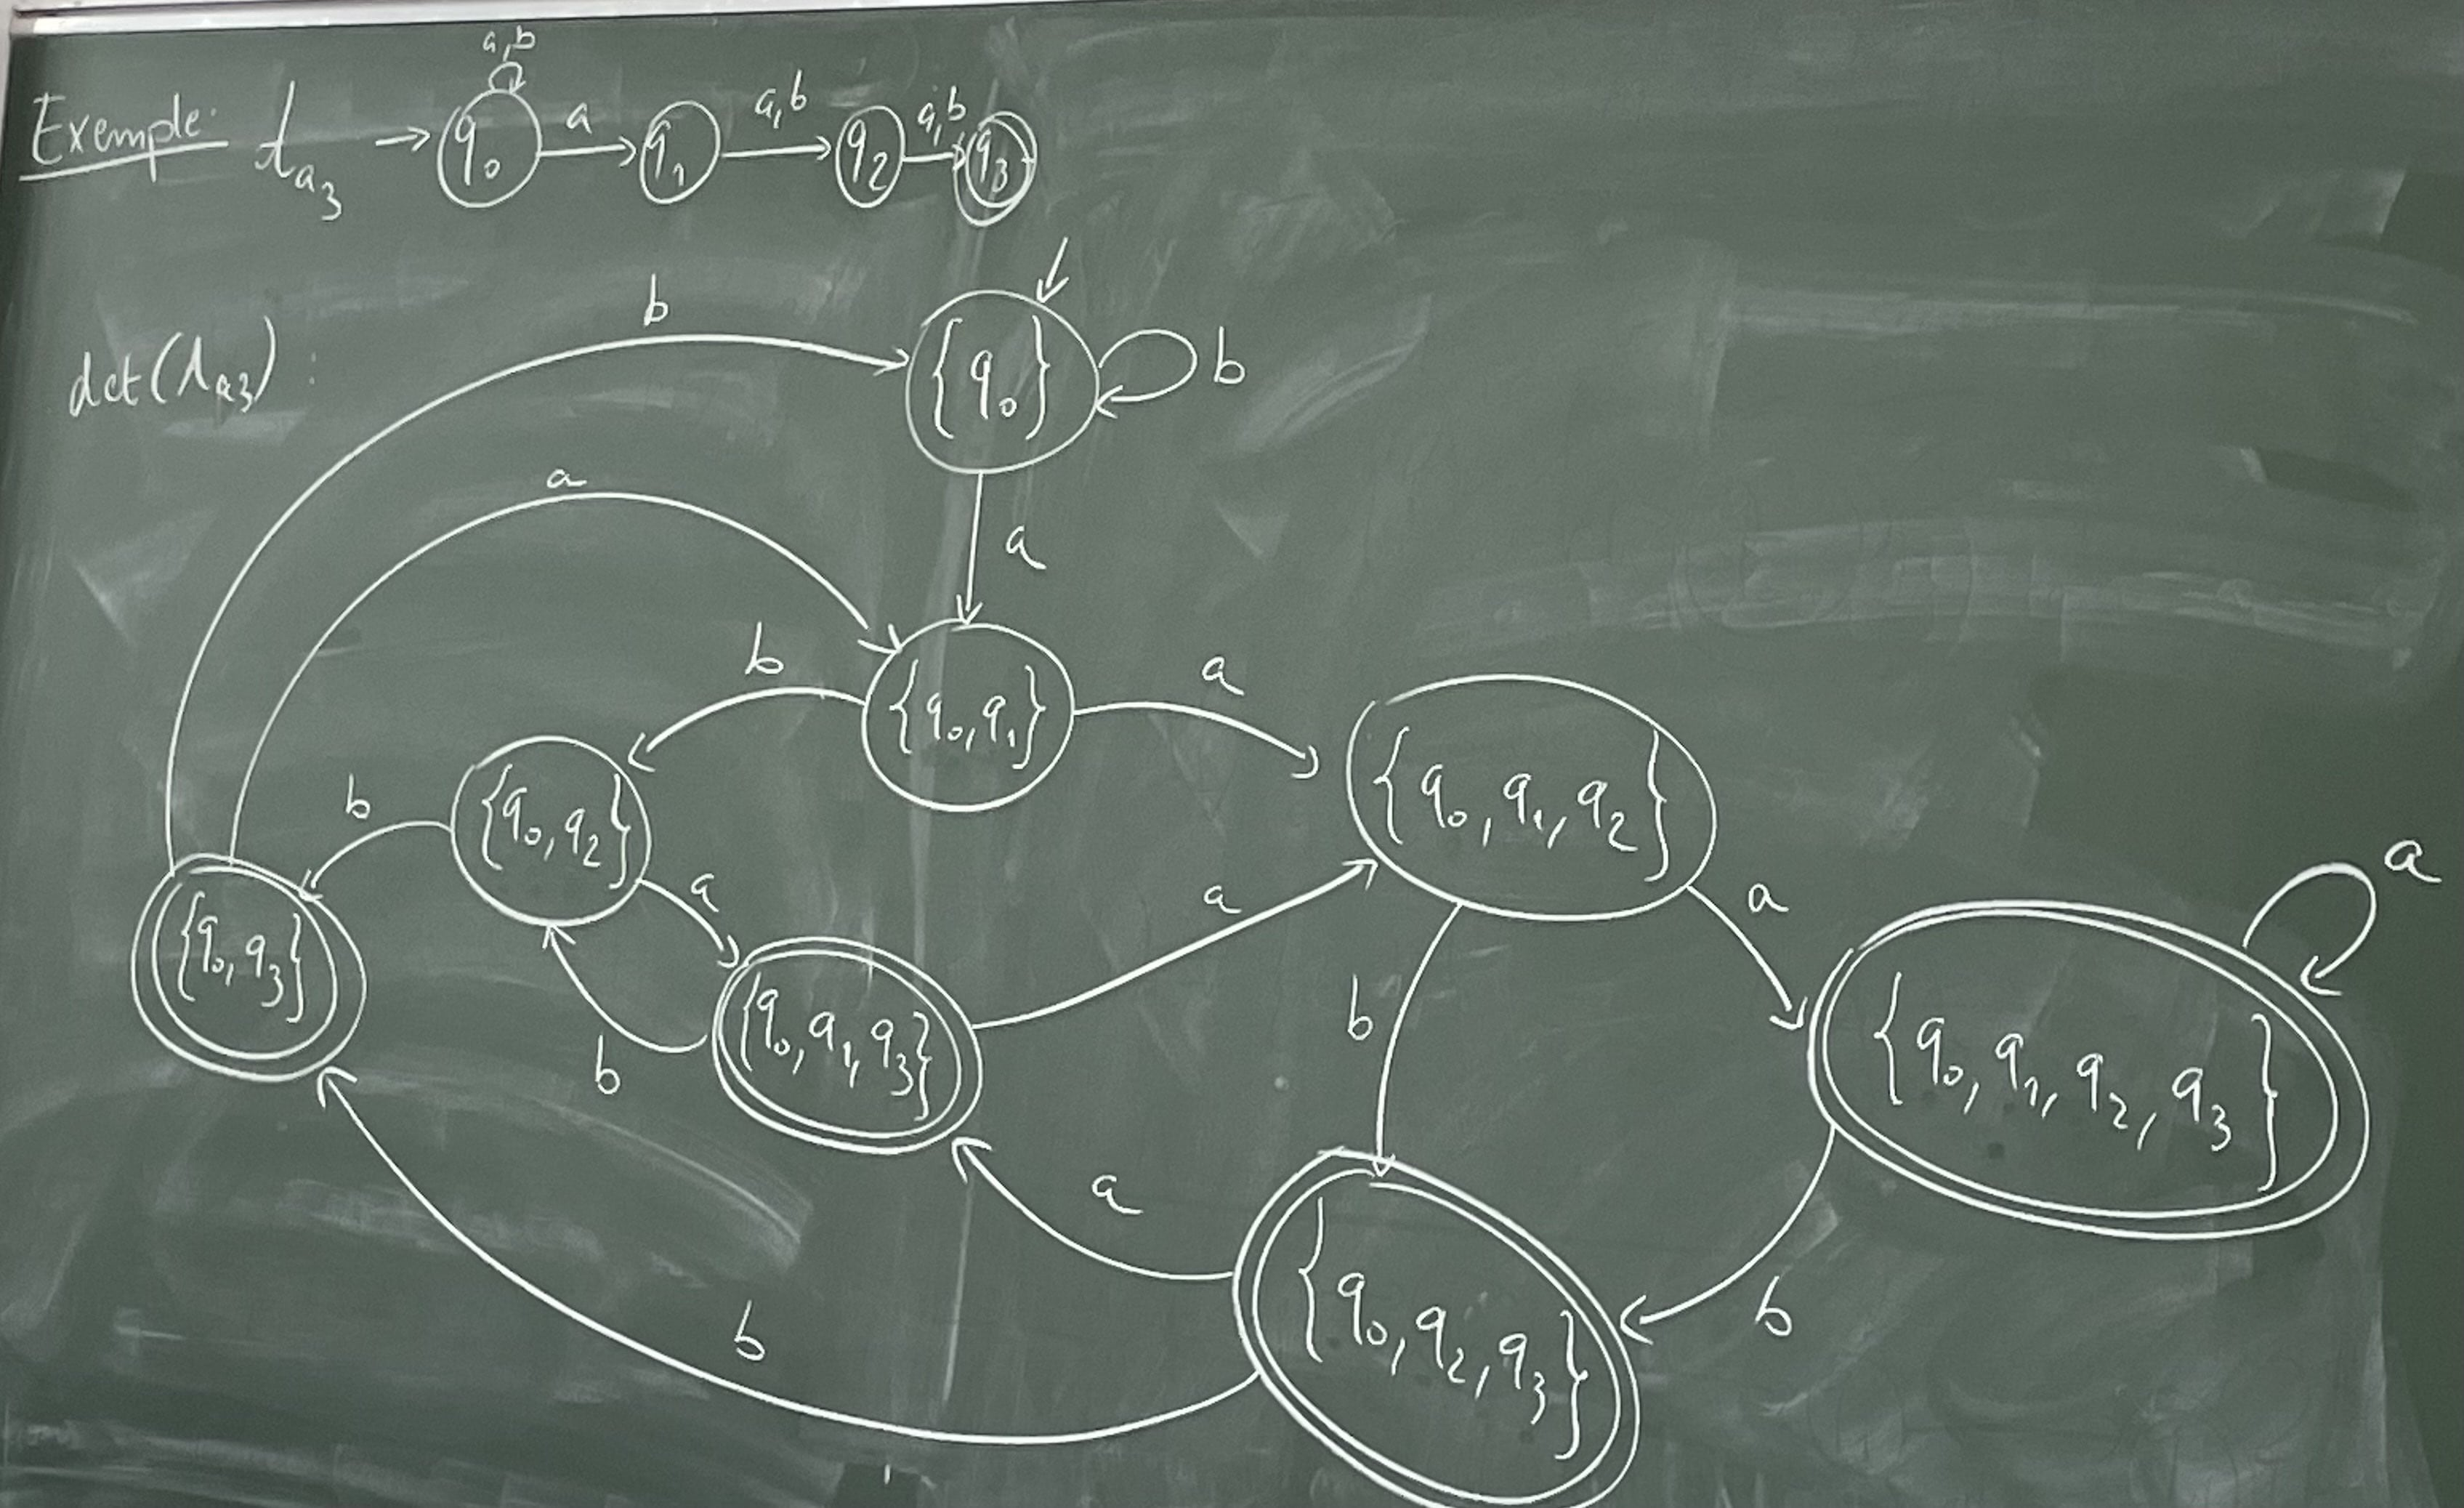
\includegraphics[scale=0.1]{Dessin/Gros_dessin.jpeg}
    \end{example}
    
    \begin{theorem}{}{}
        Soit $\bcA_N = \p{Q_N, \Sigma, q_0, F_n, \delta_n}$ un NFA.
        On a $\bcL\p{\bcA_n} = \bcL\p{\det\p{\bcA_n}}$
    \end{theorem}
    
    \begin{nproof}
        Montrons que $\forall v \in \Sigma^\star$ et $r_0 \to r_1 \to \dots \to r_n$ l'unique chemin dans $\det \p{\bsA_n}$ pour $v$ (avec $R_0 = \ens{q_0}$), on a $R_n = \ens{q \in Q_n \enstq \exists q_0 \lima{v}{\bsA_n^\star} q}$.
        
        Par récurrence sur $\mod{v}$ :
        %
        \begin{enumerate}
            \itt si $\mod{v} = 0 : v = \epsilon$ donc $R_0 = \ens{q_0}$, alors c'est bon.
            
            \itt $\mod{v} = n + 1$ : Supposons la propriété vraie pour tout mot de taille $n$ Montrons qu'elle est vraie pour $v$ :
            
            $v = ua$ avec $\mod{u} = n$ et $a \in \Sigma$.
            
            Soit $R_0 \lima{u}^\star R_n \lima{a} R_{n+1}$ dans $ \det{\bsA_n}$.
            
            Par hypothèse de récurrence, $R_n = \ens{q \in Q_n \enstq \exists q_0 \lima{u}{\bsA_n^\star} q}$
            
            Par définition de $\delta_\bsD$ :
            $R_{n+1} = \delta_\bsD \p{R_n, a} = \bigcup_{q \in R_n} \delta_n \p{q, a} = \ens{q' \ in Q_n \enstq \exists \lima{v}{\bsA_n}^\star q'}$
            
            \itt On a fait toutes les positions des chemins : $q_0 \lima{u}{\bsA_n}^\star q'$
        
        
        
            Par définition de $F_d$
            
            \begin{align*}
                v \in \bcL\p{\det{A_n}} &&\iff&& \ens{q_0} \lima{v^\star} R_n &&\text{avec} \ R_n \cap F_n \neq \emptyset\\
                &&\iff&& \exists q_0 \lima{v}^\star_{\bcA_n} q &&\text{avec} q \in F_n
            \end{align*}
            
        \end{enumerate}
    \end{nproof}
    
    \begin{corollary}{}{}
        Soit $L \subseteq \Sigma^\star$ un langage : L est reconnaissable par un DFA si et seulement si L est reconnaissable par un NFA.
    \end{corollary}
    
    \begin{nproof}
        ($\Leftarrow$<=) Si $L = \bsL \p{\bsA_n}$ avec $\bsA_n$ DFA alors $L = \bsL \p{\bsA_\bsD}$ avec $\bsA_\bsD = det \p{\bsA_n}$
        ($\rightarrow$=>) Si $\bsA_\bsD = \p{Q, \Sigma, q_0, F, \delta_\bsD}$ un DFA tq $L = \bsL \p{\bsA_\bsD}$
        Alors$\bsA_n = \p{Q, \Sigma, q_0, F, \delta_n}$ avec $\delta_n \p{q, a} = \ens{\delta_\bsD \p{q, a}}$ pour tout $q \in \alpha, a \in \Sigma$ vérifie $L \in \bsL \p{\bsA_n}$
    \end{nproof}
    
    On va maintenant montrer comment supprimer les $\epsilon$-transitions.
    
    \begin{definition}{$\epsilon$-fermeture}{}
        Soit $\bsA = \ens{Q, \Sigma, q_0, F, \delta}$ un $\epsilon$-NFA. 
        Soit $q\in Q $ %une ligne
        
        on appelle $\varepsilon$-fermeture de q l'ensemble: 
        
        %remy a supprimer la formule
        
    \end{definition}
    \begin{notation}
        Si $Q' \subseteq \text{  , } E(Q') = \bigcup E(q) $ 
        
    \end{notation}
    
    %manque 1 definition, 1 notation, 1 theoreme, 1 corrolaire, 1 definition 
    
    \subsection{Theoreme de Kleeme}
    
    \begin{theorem}{de Kleeme}{}
    Soit $\Sigma$ un alphabet 
    
    
    $Rcc_\Sigma = Reg_\Sigma$
    
    %il manque un gros paragraphe 
    
    \end{theorem}
    
    \subsubsection{Construction de Thompson}
    
    \begin{definition}{automates de Thomposon}{}
        
    \end{definition}
    
    \begin{nproof}{Par induction}
        plein de petite dessin par millier 
        
    \end{nproof}
    
    On remarquera que dans les automates de \textsc{Thompson}, on a souvent la situation suivante :
    %
    \begin{tikzpicture}
        
    \end{tikzpicture}
    %
    En réalité, les \guill{vrais} états initiaux sont $q_{i_1}, \dots, q_{i_n}$ mais notre définitions des automates impose d'avoir un seul état initial. Dans la définitions des NFA, on peut en fait autoriser un ensemble $I \subseteq Q$ d'états initiaux au lieu d'un unique $q_0$. Dans ce cas, pour l'automate des parties (algorithme pour déterminer un NFA), il faut choisir $I$ à la place de $\ens{q_0}$ pour l'état initial.
    
    \begin{theorem}{}{}
        Soient \hg{$\Sigma$ un alphabet} et \hg{$r$ une expression régulière} sur $\Sigma$. On a :
        %
        \[ \hg{\bcL\p{\th r} = \bcL\p{r}}\]
    \end{theorem}
    
    \begin{nproof}
        Soient $\Sigma$ un alphabet et $r$ une expression régulière sur $\Sigma$. On procède par induction structurelle sur $r$. Traitons d'abord les cas de base :
        %
        \begin{enumerate}
            \itt Si $r = \emptyset$, on a $\th r = \th \emptyset = $ dessin.
            
            Dans ce cas, $\bcL\p{\th r}\bcL\p{\th \emptyset} = \emptyset = \bcL\p{\emptyset} = \bcL\p{r}$.
            
            \itt Si $r = \epsilon$, on a $\th r = \th \epsilon = $ dessin.
            
            Dans ce cas, $\bcL\p{\th r} = \bcL \p{\th \epsilon} = \ens{\epsilon} = \bcL\p{\epsilon} = \bcL\p{r}$
            
            \itt Si $r = a$, on a $\th r = \th a = $ dessin.
            
            Dans ce cas, $\bcL\p{\th r} = \bcL \p{\th a} = \ens{a} = \bcL\p{a} = \bcL\p{r}$
        \end{enumerate}
        %
        Pour l'induction, on considère $r_1$ et $r_2$ deux expressions régulières telles que :
        %
        \[ \bcL\p{\th r_1} = \bcL\p{r_1} \qquad\et\qquad \bcL\p{\th r_2} = \bcL\p{r_2} \]
        %
        On pose $A_1 = \th r_1$ et $A_2 = \th r_2$. Traitons alors les différentes règles d'induction, en considérant un $r$ obtenu à partir de $r_1$ et $r_2$. On pose directement $A = \th r$. On a :
        %
        \begin{enumerate}
            \itt Si $r = r_1r_2$, alors :
            %
            \[ A :\quad \to q_1 \lima{\epsilon} q_i^1 A_1 q_f^1 \lima{\epsilon} q_i^2 A_2 q_f^2 \lima{\epsilon} q_f\]
            %
            Soit $v \in \bcL\p{r_1r_2}$, alors il existe $v_1 \in \bcL\p{r_1}$ et $v_2 \in \bcL\p{r_2}$. Par hypothèse, on a donc $v_1 \in \bcL\p{A_1}$ et $v_2 \in \bcL\p{A_2}$.
            
            Puisque $v_1 \in \bcL\p{A_1}$, il existe un chemin $q_i^1 \lima{v_1}_{A_1}^\star q_f^1$.
            
            De même, $v_2 \in \bcL\p{A_2}$, il existe un chemin $q_i^2 \lima{v_2}_{A_2}^\star q_f^2$.
            
            Donc :
            %
            \[ q_i \lima{\epsilon} q_i^1 \lima{v_1}{}_A^\star q_f^1 \lima{\epsilon}  q_i^2 \lima{v_2}{}_A^\star q_f^2 \lima{\epsilon}  q_f\]
            %
            Donc $\epsilon v_1 \epsilon v_2 \epsilon \in \bsL \p{A}$
        (car $\epsilon v_1 \epsilon v_2 \epsilon = v_1 v_2 = v$)
        ainsi $\bsL\p{r_1r_2} \subseteq \bsL(A)$ 
            
        
        Réciproquement, si $v\in \bsL(\bcA)$, forcément le chemin acceptant $v$ dans $\bcA$ est de la forme précédente, donc $v= \epsilon v_1 \epsilon v_2  \epsilon $
        
        
        Donc $v = v_1v_2$ avec $v_1 \in \bcL\p{A_1} = \bcL\p{r_1}$ et $v_2 \in \bcL\p{A_2} = \bcL\p{r_2}$ d'où $v \in \bcL\p{r_1r_2}$, ainsi $\bcL\p{A} \subseteq \bcL\p{r_1r_2} = \bcL\p{r}$.
        
            \itt Si $r = r_1 \vert r_2$, alors :
            
            \textcolor{magenta}{DESSIN}
            
            Soit $v \in \bcL\p{r_1 \vert r_2}$. Par hypothèse d'induction, on a $v \in \bcL\p{A_1}$ donc $q_i^1 \lima{v}_{A_1}^\star q_f^1$. Par construction, 
            %
            \[ q_i \lima{\epsilon} q_i^1 \lima{v}_A^\star q_1^f \lima{\epsilon} q_f\]
            %
            accepte $v$ dans $A$, donc $v \in \bcL\p{A}$, d'où $\bcl\p{r_1 \vert r_2} \subseteq \bcL\p{\bcA} = \bcL\p{\th r}$.
            
            Réciproquement, si $v \in \bcL\p{A}$, alors son chemin acceptant est de la forme :
            %
            \[ q_i \lima{\epsilon} q_i^1 \lima{v}_{A}^\star q_f^1 \lima{\epsilon} q_f \qquad\ou\qquad TODO\]
            %
            Donc $v \in \bcL\p{A_1}$ ou $v \in \bcL\p{A_2}$. Par hyptohèse d'induction, $v \in \bcL\p{r_1} \cup \bcL\p{r_2} = \bcL\p{r_1 \vert r_2}$.
            
            \itt Si $r = r_1^\star$, alors :
            %
            \textcolor{magenta}{\Huge{DESSIN}}
            %
            Soit $v \in \bcL\p{r_1^\star} = \bcL\p{r_1}^\star$. Il existe un entier $m \in \bcN$ tel que $v = v_1 \dots v_m$ avec $v_i \in \bcL\p{r_1}$ pour $i \in \iint{1, m}$.
            
            Montrons par récurrence sur m que $v \in \bsL \p{A}$ :
            \begin{enumerate}
                \ithand Si $m = 0$, alors $v = \epsilon \in \bsL \p{A}$ car $q_i \lima{\epsilon} q_i^1 \lima{\epsilon} q_f^1 \lima{\epsilon}  q_f$
                    
                \ithand Si $m \geq 1$, alors par hypothèse de récurrence, $v_1\cdots v_{n+1} \in \bcL\p{A}$. Donc :
                %
                \[ q_i \lima{\epsilon} q_i^1 \lima{v_1\dots v_{n-1}}_A^\star q_f^1 \lima{\epsilon} q_f\]
                %
                Or $v_m \in \bcL\p{r_1} = \bcL\p{A_1}$ soit l'hypothèse de récurrence. Ainsi $q_i^1 \lima{v_m}_{A_1}^\star q_f^1$.
            \end{enumerate}
                
            Donc $v$ est accepté dans $A$ par:    
            %
            \[ q_i \lima{\epsilon} q_i^1 \lima{v_1 \dots v_{m-1}}_A^\star q_f^1 \lima{\epsilon} q_i^1 \lima{v_m}_A^\star q_f^1 \lima{\epsilon} q_f \]
            %
            Donc $v \in \bcL\p{A}$. Réciproquement, soient $v \in \bcL\p{A}$ et $q_i \lima{v}_A^\star q_f$ acceptant $v$.
            %
            \begin{enumerate}
                \ithand Si $q_i \lima{\epsilon} q_i^1 \lima{\epsilon} q_f^1 \lima{\epsilon} q_f$, alors 
                
                \ithand 
                
                \ithand sinon, on peut toujours se ramener à un chemin n'ayant pas de morceau de la forme :
                %
                \[ q_i \lima{\epsilon} q_i^1 \lima{v_1}_{A_1}^\star q_f^1 \lima{\epsilon} q_i^1 \lima{v_2}_{A_1}^\star \lima{\epsilon} q_i^1 \lima \dots \lima{v_m}ç{A_1}^\star q_f^1 \lima{\epsilon} q_f\]
                %
                Donc $v =v_1 \dots v_m$ avec $v_i \in \bcL\p{A_1} = \bcL\p{r_1}$ pour $i \in \iint{1, m}$, donc $v \in \bcL\p{r_1^\star}$.
             \end{enumerate}
        \end{enumerate}
    \end{nproof}
    
    On remarquera que cette preuve est constructive. Elle fournit donc un algorithme qui, à partir d'une expression régulière $r$, fournit un automate reconnaissant $\bcL\p{r}$. L'automate de \textsc{Thompson} doit son nom à l'informaticien \textsc{Ken Thompson} qui a créé l'outil \texttt{grep}, reposant sur la construction des automates (de \textsc{Thompson}). 
    
    On remarquera par ailleurs que 'l'on vient de montrer que $\mathrm{Reg}_\Sigma \subset \mathrm{Rec}_\Sigma$. La section suivante propose une autre démonstration (elle aussi constructive) de cette inclusion.
    
    \subsubsection{Algorithme de Berry-Sethi, automate de Glushkov}
        
    \begin{definition}{Langage local}{}
        Soit $\Sigma$ un alphabet, et $L \subset \Sigma^\star$ un langage. On note :
        %
        \begin{enumerate}
            \itast $\First\p{L} = \ens{a \in \Sigma \enstq \ens{a}\Sigma^\star \cap L \neq \emptyset}$
            
            \itast $\Last\p{L} = \ens{a \in \Sigma \enstq \Sigma^\star\ens{a} \cap L \neq \emptyset}$
            
            \itast FACTS
            
            \itast NFACTS
        \end{enumerate}
    \end{definition}
    
    \begin{example}
            exemple triviale 
            
            
            
            Soit $v \in (First(L1)\Sigma $ %remy ecrit %LOL NON TA CRU
            
            
    \end{example}
    
    \begin{definition}{automate de Glushkov}{}
        Soit $\Sigma$ un alphabet et $L \subset \Sigma^\star$ un langage local. On appelle \hg{automate de \textsc{Glushkov}} de $L$ l'automate $\Loc{L} = \p{Q_L, \Sigma, q_0, F_L, \delta_L}$ tel que :
        %
        \begin{enumerate}
            \itast $Q_L = \ens{q_0} \cup \ens{q_a \enstq a \in \Sigma}$
            
            \itast $F_L = \ens{q_a \enstq a \in \Last{L}} $
        \end{enumerate}
        
        
    \end{definition}
    
    \begin{theorem}
        Soit $\Sigma$ un alphabet et $L \subseteq \Sigma^\star$ un langage local. $L = \bcL(Loc(L))$
    \end{theorem}
    \begin{nproof}
        L $\subset \bsL(Loc(L))$
        \begin{enumerate}
            \itt \Huge{blablablablbalbal}
        \end{enumerate}
    \end{nproof}
    
    \begin{definition}{Expression linéaire}{}
        Soit \hg{$\Sigma$} un \hg{alphabet}. Une \hg{expression régulière} sur $\Sigma$ est dite \hg{linéaire} lorsque \hg{tout symbole de $\Sigma$ y apparaît au plus une fois}.
    \end{definition}
    
    On a les exemples ci-dessous :
    %
    \begin{example}{}{}
        Considérons l'alphabet $\Sigma$ tel que $\ens{a, b, c} \in \Sigma$.
        \begin{enumerate}
            \itt \hg{$a^\star bc^\star$} est une expression régulière.
            
            \itt \hg{$ba^\star bc^\star b$} n'est \hg{pas} une expression régulière.
        \end{enumerate}
    \end{example}
    
    Montrons d'abord le lemme suivant :
    %
    \begin{lemma}{}{}
        Soient \hg{$\Sigma_1$} et \hg{$\Sigma_2$} deux \hg{alphabets} tels que \hg{$\Sigma_1 \cap \Sigma_2 \neq \emptyset$}, ainsi que \hg{$\bcL_1$} et \hg{$\bcL_2$} deux \hg{langages locaux}, respectivement \hg{sur $\Sigma_1$} et \hg{sur $\Sigma_2$}. Dans ce cas :
        %
        \begin{enumerate}
            \itast \hg{$\bcL_1 \cap \bcL_2$} est un \hg{langage local sur $\Sigma_1 \cap \Sigma_2$} ;

            \itast \hg{$\bcL_1 \cup \bcL_2$} est un \hg{langage local sur $\Sigma_1 \cup \Sigma_2$} ;
            
            \itast \hg{$\bcL_1 \cdot \bcL_2$} est un \hg{langage local sur $\Sigma_1 \cup \Sigma_2$} ;
            
            \itast \hg{$\bcL_1^\star$} est un \hg{langage local}.
        \end{enumerate}
    \end{lemma}
    
    \begin{nproof}
        Soient $\Sigma_1$ et $\Sigma_2$ deux alphabets tels que $\Sigma_1 \cap \Sigma_2 \neq \emptyset$, $\bcL_1$ un langage local sur $\Sigma_1$ et $\bcL_2$ un langage local sur $\Sigma_2$.
        
        On note pour \(i\in \ens{1, 2}\) : \(La_i =\) Last(\(L_i\)), \(Fi_i =\) First(\(L_i\)), \(Fa_i =\) Fact(\(L_i\)), \(NFa_i\) = NFact(\(L_i\))

        \begin{psse}
            \item Si \(v \in \left(\bcL_1\cap\bcL_1\right)\backslash\ens{\varepsilon}\) alors \(v = a_i \hdots a_n\) avec \(a_1 \in Fi_1 \cap Fi_2\) et \(a_n \in \bcL a_1 \cap \bcL a_2\) et \(\forall i, a_i a_{i+1} \in Fa_1 \cap Fa_2\)

            Et réciproquement, tout mot vérifiant ces trois propriétés est dans les langages car ils sont locaux. donc en posant \(Fi = Fi_1 \cap Fi_2\), \(La = La_1 \cap La_2\) et ainsi de suite on a go 
            \[ \left(\bcL_1\cap \bcL_2 \right) \backslash \ens{\varepsilon} = \left(Fi\Sigma^{\alpha} \cap \Sigma^{\alpha} \bcL a\right) \backslash \Sigma^{\alpha} NFa \Sigma^*\]

            On vérifie facilement que les nouveaux ensembles sont les caractéristiques de \(\bcL=\bcl_1\cup\bcL_2\)
            
            Donc $L \backslash \ens{\varepsilon} \subseteq \quad (F_i \Sigma^* \cap \Sigma^* $

            \item Réciproquement  si \(v\in \bcL\backslash\ens{\varepsilon}\), alors :
            %
            $v = a_1\dots a_n$ et si $a_1 \in F_{i_1}$, donc $a_1 \in \Sigma_1$.
            
            Donc $a_1a_2 \in F_{a_1}$ (car $\Sigma_1 \cap \Sigma_2 \neq \emptyset$).
            
            Donc $a_2 \in \Sigma_1$, \dots
            
            On montre de proche en proche (car $\Sigma_1 \cap \Sigma_2 \neq \emptyset$) que $v \in \Sigma_1^\star$ et que pour tout $i \in \iint{1, n-1}$, $a_ia_{i+1} \in F_{a_1}$. De plus, $a_1 \in \bcL_\epsilon  = \bcL_{a_1} \cup \bcL_{a_2}$.
            
            Or $a_n \in \Sigma_1$ donc $a_n \in \bcL_{a_1}$. Donc $v \in \bcL_1$ (car $\bcL_1$ est local) d'où $v \in \bcL$.
            
            Si $a_1 \in F_{i_2}$, on montre de manière similaire que $v \in \bcL_2$, donc que $v \in \bcL$. Au final, $\bcL' \backslash \ens{\epsilon} \subseteq \bcL \backslash \ens{\epsilon}$, et donc $\bcL$ est un langage local.
            
            \item Notons $\bcL = \bcL_1 \cdot \bcL_2$. Les ensembles caractéristiques de $\bcL$ sont $\bcF_i = \left\lbrace \begin{array}{ll}
                \bcF_{i_1} &\text{si} \ \epsilon \not\in \bcL_1  \\
                \bcF_{i_1} \cup \bcF_{i_2} &\text{sinon} 
            \end{array}\right.$ et $\bcL_a = \left\lbrace \begin{array}{ll}
                \bcL_{a_2} &\text{si} \ \epsilon \not\in \bcL_2  \\
                \bcL_{a_1} \cup F_{a_2} &\text{sinon} 
            \end{array}\right.$.
            
            On a $\bcF_a = \bcF_{a_1} \cup \bcF_{a_2} \cup \p{\bcL_{a_1} \cdot \bcF_{i_2}}$ donc on a bien $\bcL \backslash \ens{\epsilon} \subseteq \underbrace{\p{\bcF_i \Sigma^\star \cap \Sigma^\star L_a} \backslash \Sigma^\star NF_\alpha \Sigma^\star}_{\bcL'}$.
            
            Soit $v \in \bcL' \backslash \ens{\epsilon}$. On a $v = a_1 \dots a_n$, et :
            %
            Si $a_1 \in \bcF_{i_2}$, alors $\epsilon \in \bcL_1$. Comme $\Sigma_1 \cap \Sigma_2 \neq \emptyset$, on montre, comme dans le cas précédent de proche en proche, que $v \in \Sigma_2^\star$ et que pour tout $i \in \iint{1, n-1}$ on a $a_ia_{i+1} \in \bcF_{a_2}$ et $a_n \in \bcL_{a_2}$. Ainsi, $v \in \bcL_2$ car le langage est local.
            
            Or $\epsilon \in \bcL_1$ donc $v \in \bcL = \bcL_1 \cdot \bcL_2$.
            
            Si $a_1 \in F_{i_1}$, soit $a_1 \dots a_p$ le plus long préfixe de $v$ dans $\Sigma_1^\star$. On a:
            \begin{enumerate}
                \itt $a_1$ \in $\bcF_{i_1}$ ;
                
                \itt $\forall i \ in [|1, p-1|] a_i a_{i+1} \in F_{a1} $%va y 
                
                \itt montrons que $a_p \in \bcL_{a_1}$ : si $p = n$, on a $a_p \in \bcL_a \cap \Sigma_1 = \bcL_{a_1}$ et forcément $\epsilon \in $ ....

                Donc $v= \underbrace{a_1 \dots a_p}_{\in \bcL_1} \underbrace{a_{a+1} \dots a_n}_{\in \bcL_2} \in L_1 \cdot L_2$, d'où $L_1\cdot L_2$ est local.
                
            \end{enumerate}     
            
            \item Notons $\bcL = \bcL_1^\star$. On a $\bcF_i = \bcF_{i_1}$, $\bcL_a = \bcL_{a_1}$ et $\bcF_a = \bcF_{a_1} \cup \p{\bcL_{a_1} \cdot \bcF_{i_1}}$.
                
            On a bien $\bcL \backslash \ens{\epsilon} \subseteq L'$.
                
                Soit $v \in L' \backslash \ens{\epsilon} $
                %il effacer le tableau

        \end{psse}
    \end{nproof}
    
    
    \begin{property}{}{}
        Soient \hg{$\Sigma$} un \hg{alphabet} et \hg{$r$} une \hg{expression régulière} sur $\Sigma$.
        %
        \[ \hg{\text{Si} \ r \ \text{est linéaire, alors} \ \bcL\p{r} \ \text{est local.}} \]
    \end{property}
    
    \begin{nproof}
        Soient $\Sigma$ un alphabet et $r$ une expression régulière sur $\Sigma$.
        %
        \begin{enumerate}
            \itt Si \(r = \emptyset : \bcL(r) = \emptyset\) est bien local
            \itt Si \(r= \epsilon : \bcL(\epsilon) = \ens{\epsilon}\) est bien local
            \itt Si \(r=a, \bcL(a) = \ens{a}\) est bien local

            \itt Si \(r = r_1 \mid r_2\) avec par hypothèse d'induction \(r_1\) et \(r_2\) locaux, comme \(r\) est linéaire on a que \(r_1\) et \(r_2\) sont distincts donc par lemme(2) \(\bcL(r) = \bcL(r_1)\cup\bcL(r_2)\)

            \itt Si \(r = r_1 \cdot r_2\) par hypothèse d'induction \(\bcL(r_1)\) et \(\bcL(r_2)\) sont locaux et par linéarité de \(r\) les deux alphabets sont distincts donc \(\bcl(r_1\cdot r_2) = \bcL(r_1) \cdot \bcL(r_2)\) par lemme (3) donc le langage est local.

            \itt Si \(r = r_1^*\) par hypothèse d'induction \(\bcL(r_1)\) est local et par lemme (4) \(\bcL(r_1^*) = \bcL(r_1)^*\) est local.
        \end{enumerate}
    \end{nproof}
    
    \begin{definition}{Linéarisation}
        Si r est une expression régulière sur $\Sigma$ on peut le transformer en une 
        expression régulière linéaire linéaire sur $\Sigma'$ avec le processus suivant
        \begin{enumerate}
            \itast On initialise \(\Sigma' = \emptyset\)
            \itast On lit \(r\) de gauche à droite 
            \itast Si \(a\in\Sigma\) est la \(i\)-ème lettre de \(r\) on la remplace par une lettre notée \(a_i\) qui ajoute \(a\) dans \(\Sigma'\)
        \end{enumerate}
    \end{definition}
    
    \begin{example}{}{}
        Considérons l'expression régulière \hg{$r$} sur l'alphabet $\hg{\Sigma = \ens{a, b}}$ suivante :
        %
        \[ \hg{r = a\p{ab}^\star \vert b^\star a}\]
        %
        On \hg{linéarise $r$ en l'expression $r'$} sur $\hg{\Sigma' = \ens{a_1a_2b_3b_4a_5}}$ :
        %
        \[ \hg{r' = a_1\p{a_2b_3}^\star \vert b^4a_5 } \]
    \end{example}
    
    \begin{form}{Algorithme de Berry-Sethi}{}
        Soient \hg{$\Sigma$} un \hg{alphabet} et $r$ une \hg{expression régulière} sur $\Sigma$. L'\hg{algorithme de \textsc{Berry-Sethi}} consiste à :
        
        \begin{psse}
            \item \hg{linéariser $r$} en \hg{$r'$} ;
            
            \item \hg{calculer $\First{\bcL\p{r'}}$}, \hg{$\Last{\bcL\p{r'}}$} et \hg{$\Fact{\bcL\p{r'}}$} ;
            
            \item \hg{construire $\bcA = \Loc{\bcL\p{r'}}$} ;
            
            \item \hg{effacer} les \hg{indices des symboles} dans les \hg{transitions de $\bcA$}.
        \end{psse}
    \end{form}
    
    \begin{notation}
        Si \hg{$\bcA = \left( Q,\Sigma',q_0,F,\delta'\right)$} on obtient d'après l'étape \pssenum{iv} : 
        %
        \[ \hg{f\p{\bcA} = \p{Q,\Sigma,q_0,F,\delta}} \qquad\text{où}\qquad \forall \p{q, a_i} \in \mathrm{dom}{\delta'},\qquad \delta\p{q,f(a_i)} = \delta'\p{q,a_i}\]
    \end{notation}
    
    \begin{theorem}{}{}
        Soit $r$ une expression régulière sur $\Sigma$. A la fin de l'algorithme de \textsc{Berry-Sethi}, on obtient un automate $f\p{\bcA}$ tel que $\bcL\p{r} = \bcL\p{f\p{\bcA}}$.
    \end{theorem}
    
    \begin{nproof}
        D'après les résultats précédents, $r'$ est linéaire, donc $\bcL\p{r'}$ est local, doc $\bcA = \Loc\p{\bcL\p{r'}}$ vérifie $\bcL\p{\bcA} = \bcL\p{r'}$, avec $f\p{r'} = r$. Montrons que $\bcL\p{f\p{A}} = \bcL\p{r}$ par double inclusion.

        \begin{enumerate}
            \itt $\boxed{\supseteq}$ Soit $u \in \bcL\p{r}$. Si $u \in \bcL\p{r'}$, alors $\epsilon \in \bcL\p{r'}$, donc $\epsilon \in \bcL\p{\bcA}$. Dès lors, $q_0 \in \bcF$, d'où $\epsilon \in \bcL\p{\bcF\p{A}}$.
            
            Sinon, on a $u = u_1\dots u_n$, et donc il existe $u' \in \bcL\p{r'}$ tel que $u = f\p{u'}$. Ici $u' \in \bcL\p{\bcA}$, donc il existe un chemin dans $\bcA$ : \qquad $q_0 \xrightarrow{u_1'} q_1 \xrightarrow{u_2'} q_2 \dots \xrightarrow{u_n'} q_n \in F$. Ainsi 
            %
            \[ q_0 \xrightarrow{f\p{u_1'}} q_1 \xrightarrow{f\p{u_2'}} q_2 \dots \xrightarrow{f\p{u_n'}} q_n \in F \qquad \text{est un chemin dans} \ f\p{A}\]
            %
            Donc le chemin : \qquad $q_0 \xrightarrow{f\p{u_1}} q_1 \xrightarrow{f\p{u_2}} \dots \xrightarrow{f\p{u_n}} q_n$ est un chemin acceptant $u$ dans $f\p{\bcA}$, donc $u \in \bcL\p{f\p{\bcA}}$.
            
            \itt $\boxed{\subseteq}$ Soit $u \in \bcL\p{f\p{\bcA}}$, si $u = \epsilon$, alors $\epsilon \in \bcL\p{f\p{\bcA}}$, donc $q_0 \in \bcF$, donc $\epsilon \in \bcL\p{\bcA} = \bcL\p{r'}$ d'où $\epsilon \in \bcL\p{r}$.
            
            Sinon, $u = u_1 \dots u_n$, ainsi il existe un chemin dans $f\p{\bcA}$ :
            %
            \[ q_0 \xrightarrow{f\p{u_1}} q_1 \dots \xrightarrow{f\p{u_2}} q_2 \dots \xrightarrow{f\p{u_n}} u_n \in F\]
            %
            Pour $i \in \iint{1, n}$, la transition $q_{i-1} \xrightarrow{f\p{u_i}} q_i$ de $f\p{\bcA}$ correspond à une transition $q_{i-1} \xrightarrow{u_i} q_i$ de $\bcA$ avec $f\p{u_i'} = u_i$, donc :
            %
            \[ q_0 \xrightarrow{f\p{u_1'}} q_1 \xrightarrow{f\p{u_2'}} q_2 \dots \xrightarrow{f\p{u_n'}} q_n \in F\]
            %
            est un chemin acceptant $u' = u_1'\dots u_n'$ dans $\bcA$, donc $u' \in \bcL\p{\bcA} = \bcL\p{r'}$, et ainsi $u = f\p{u'} = \bcL\p{f\p{r'}} = \bcL\p{r}$.
        \end{enumerate}
    \end{nproof}
    
    \begin{example}{}{}
        Reprenons l'expression régulière $r$ sur l'alphabet $\hg{\Sigma = \ens{a, b}}$ précédente ($\hg{r = a\p{ab}^\star \vert b^\star a}$), qu'on avait linéarisée sur $\hg{\Sigma' = \ens{a_1a_2b_3b_4a_5}}$ en :
        %
        \[ \hg{r' = a_1\p{a_2b_3}^\star \vert b^4a_5 } \]
        %
        On obtient alors :
        %
        \begin{enumerate}
            \itt $\hg{\First{\bcL\p{r'}} = \ens{a_1, b_4, a_5}}$ ;
            
            \itt $\hg{\Last{\bcL\p{r'}} = \ens{a_1, b_3, a_5}}$ ;
            
            \itt $\hg{\Fact{\bcL\p{r'}} = \ens{a_1a_2, a_2b_3, b_3a_2, b_4a_5, b_4b_4}}$ ;
        \end{enumerate}
        %
        Ceci permet d'obtenir l'automate de $r$ :
        %
        \begin{center}
            DESSIN
        \end{center}
    \end{example}
    
    On remarque que la construction de Gluskow est donc une alternative à la 
    construction de Thompson. 
    \begin{enumerate}
        \itt L'avantage de la construction de Thompson est qu'elle est plus facile à prouver correcte. 
        
        
        \itt Concernat l'algorithme de Berry-Sethi, sa preuve de correction est moins directe, mais est très facile à faire à la main sur un example, car il a l'avantage: 
        
        \itt    de former un automate avec peu d'états (nombre de lettres dans l'expression de départ
        
        \itt    de fournir un automate sans $\varepsilon$ transition 
    
    \end{enumerate}
    
    
    
    Ces deux constructions sont liées par la propriété suivante :
    
    
    
    \begin{property}{}{}
        Soit $r$ une regex. $rm^\epsilon \p{Th\p{r}} = f\p{\bcL\p{\bcA}}$
    \end{property}
    
    \begin{nproof}
        Admise.
    \end{nproof}
    
    \subsubsection{Algorithme d'élimination des états}
    
    On montre maintenant que $Rec_\Sigma \subseteq Reg_\Sigma$, en présentant l'algorithme de Brzozowski et McCuskey. Cet algorithme repose sur une nouvelle définition d'automate.
    
    \begin{definition}{automate généralisé}{}
        Un automate généralisé est un quintuplet $A = \ens{Q, \Sigma, q_0, F, \delta}$ où
        \begin{enumerate}
            \itt $Q, \Sigma, q_0, F$ sont défini comme avant
            \itt $\delta \subseteq Q \times Reg_\Sigma \times Q$ est une relation de transition de A
        \end{enumerate}
    
    \end{definition}
    On remarque que
    \begin{enumerate}
        \itt  dans un tel automate, on a le droit d'étiqueter une transition par n'importe quelle expression régulière (plutôt que $a \in \Sigma$ ou $\epsilon$).
        \itt Utiliser une relation plutôt qu'une fonction dans la définition de $\delta$ va simplifier un peu la définition de l'algorithme qui va suivre.
    \end{enumerate}

    \begin{definition}{chemin}{}
        Soit $A = \p{Q, \Sigma, q_0, F, \delta}$ un automate généralisé, soit $v \in \Sigma^\star$. $v$ est accepté par $A$ si
        \begin{enumerate}
            \itt $\exists n \in \bcN^\star, \exists \p{v_1, \dots, v_n} \in \p{\Sigma^\star}^n$ tel que
            \begin{enumerate}
                \itt $v = v_1 \dots v_n$
                \itt il existe un chemin$q_0 \lima{r_1}{}_A q_1 \lima{r_2}{}_A \dots \lima{r_n}{}_A q_n \in F$ tel que $\forall i \in \iint{1, n}, v_i \in \bcL\p{r_i}$
            \end{enumerate}
        \end{enumerate}
        
    \end{definition}
    
    \begin{definition}{algorithme d'élimination d'états}{}
        Soit $A = \p{Q, \Sigma, q_0, F, \delta}$ un automate.
        \begin{enumerate}
            \item Créer l'automate généralisé $A' = \p{Q \cup \ens{q_i, q_f}, \Sigma, q_i, \ens{q_f}, \delta'}$ avec $\delta' = \delta \cup\ens{\p{q_i, \epsilon, q_0}} \cup \ens{\p{q, \epsilon, q_f} \enstq q \in F}$
            
            Cet automate $A'$ possède un seul état initial $q_i$ sans transition entrante, et un seul état $q_f$ sans transition sortante.
        
            \item on definis 2 procédure auxiliaires
            \begin{enumerate}
                \itt  élimination des transitions tant qu'il existe deux transitions distinctes $q \lima{r_1}{}_{A'} q'$ et $q \lima{r_2}{}_{A'} q'$ (même $q$ et $q'$, les supprimer, et rajouter $q \lima{r_1 \vert r_2}{} q'$
            
                \itt Elimination d'un état q: pour toutes $p \lima{r_1}{}_{A'} q$ et $q \lima{r_2}{}_{A'} s$ dans $\delta'$
                    \begin{enumerate}
                        \itt ajouter : $\left\lbrace\begin{array}{cl}
                            p \lima{r_1 r^\star r_2}{}_{A'} s &\text{si} \ q \lima{1'}^r q\\ %Le \\ pour sauter la ligne
                            p \lima{r_1 r_2}{}_{A'} & \text{sinon}
                        \end{array}\right.$ 
                        
                        %Ensuite tu met un environnement array : le deuxième crochet {cc} indique qu'on aura deux colonnes centrées. Si je voulais une colonne à gauche puis une colonne centrée je mettrait {lc} et si je voulais centré puis à gauche je mettrait {cl}. merci !!!
                        
                        %Donc ici on met {cl}. Et après le "&", on met la suite
                        
                        %ça en gros ça dit à gauche je vais mettre un bracket left (lbrace) et à droite rien, et le \left / \right aide à adapter la taille
                
                        \itt supprimer $p \lima{r_1}{}_{A'} q$ et $q \lima{r_2}{}_{A'} s$
                        
                        \itt supprimer q 
                    \end{enumerate}
                \end{enumerate}
            
            \item Boucle principale de l'algorithme 
                Pour chaque $q \in \emptyset$ 
                \begin{enumerate}
                    \itt éliminer toutes les transitions possibles
                    \itt éliminer l'état $q$
                \end{enumerate}
            \item Une fois que l'automate est réduit à $\to q_i \lima{r}{} q_f \quad \implies$ renvoyer $r$
        \end{enumerate}
    \end{definition}
    
    On remarque que si $\bcA$ possede plusieurs état initiaux $(I \subseteq Q)$
    
    \begin{theorem}{}{}
        A la fin de l'algorithme, $\bcL\p{A} = \bcL\p{r}$.
    \end{theorem}
    
    \begin{nproof}
        \begin{enumerate}
            \itt L'automate généralisé $A'$ vérifie initialement $\bcL\p{A'} = \bcL\p{A}$
            \itt On montre facilement qu'à chaque étape de l'algorithme, la modification effectuée sur $A'$ ne change pas $\bcL\p{A'}$.
            \begin{enumerate}
                \itt élimination des transitions : pour tout mot $v \in \Sigma^\star$ tq$q \lima{v}{}_{A'}^\star q'$, 
                \begin{enumerate}
                    \itt si ce chemin n'utilise pas $q \lima{r_1}{} q'$ ou $q \lima{r_2}{}q'$, alors ce chemin existe toujours après la modification
                    \itt si ce chemin utilise $q \lima{r_1}{} q'$ ou $q \lima{r_2}{}q'$, alors $v \in \bcL\p{}r_1$ ou $v \in \bcL\p{r_2}$
                    Donc $v \in \bcL\p{r_1 \vert r_2}$
                    Donc après la modification, on peut lire v en prenant $q \lima{r_1 \vert r_2}{} q'$
                    \itt Réciproquement, si $q \lima{v}{}_{A'}^\star q'$, après la modification
                    \begin{enumerate}
                        \itt si on n'utilise pas la nouvelle transition : même chemin avant le motif
                        \itt si on utilise $q \lima{r_1 \vert r_2}{} q'$ alors $v \in \bcL\p{r_1 \vert r_2}$, et qu'on pouvait lire $v$ avant le motif avec $q \lima{r_1}{} q'$ ou $q \lima{r_2}{} q'$
                    \end{enumerate}
                \end{enumerate}
                \itt élimination d'un état q :
                % INSERT IMAGE TABLEAU DE GAUCHE
            \end{enumerate}
            \itt De plus, l'algorithme termine, car le nombre de transition et d'états diminue strictement. Ainsi, à la fin, on a  $A'$ de la forme : $\to q_i \lima{r}{} q_f$ et $\bcL\p{A'} = \bcL\p{r} = \bcL\p{A}$
        \end{enumerate}
    
    \end{nproof}
    
    \begin{corollary}{}{}
        Soit $\Sigma$ un alphabet 
        $Rec_\Sigma \subseteq Reg_\Sigma$
    \end{corollary}
    
    \begin{example}{detaille de l'algo }{}
        %j'ai pris des photo de l'exemple 
        %\begin{enumerate}
            %\itt enumeration de $q_0$ : %sous shéma
            %\itt nnouvelles transitions : %sous shéma
            %On obtient : %sous-shéma
        %\end{enumerate}
        
        dessin:
        
        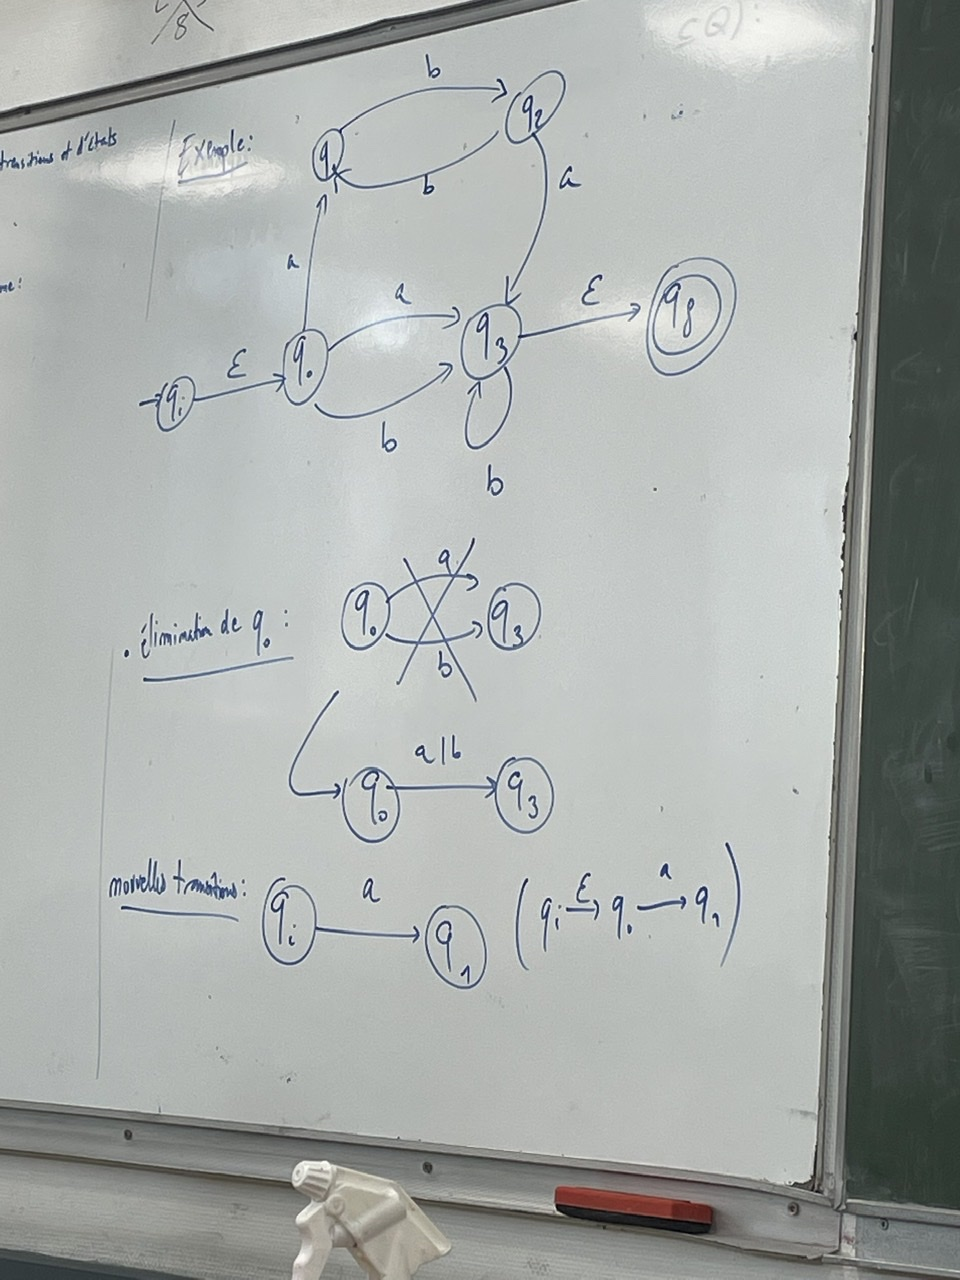
\includegraphics[scale=0.2]{Dessin/Tableau1.jpeg}%giga compresser 
        \vspace{2cm}
        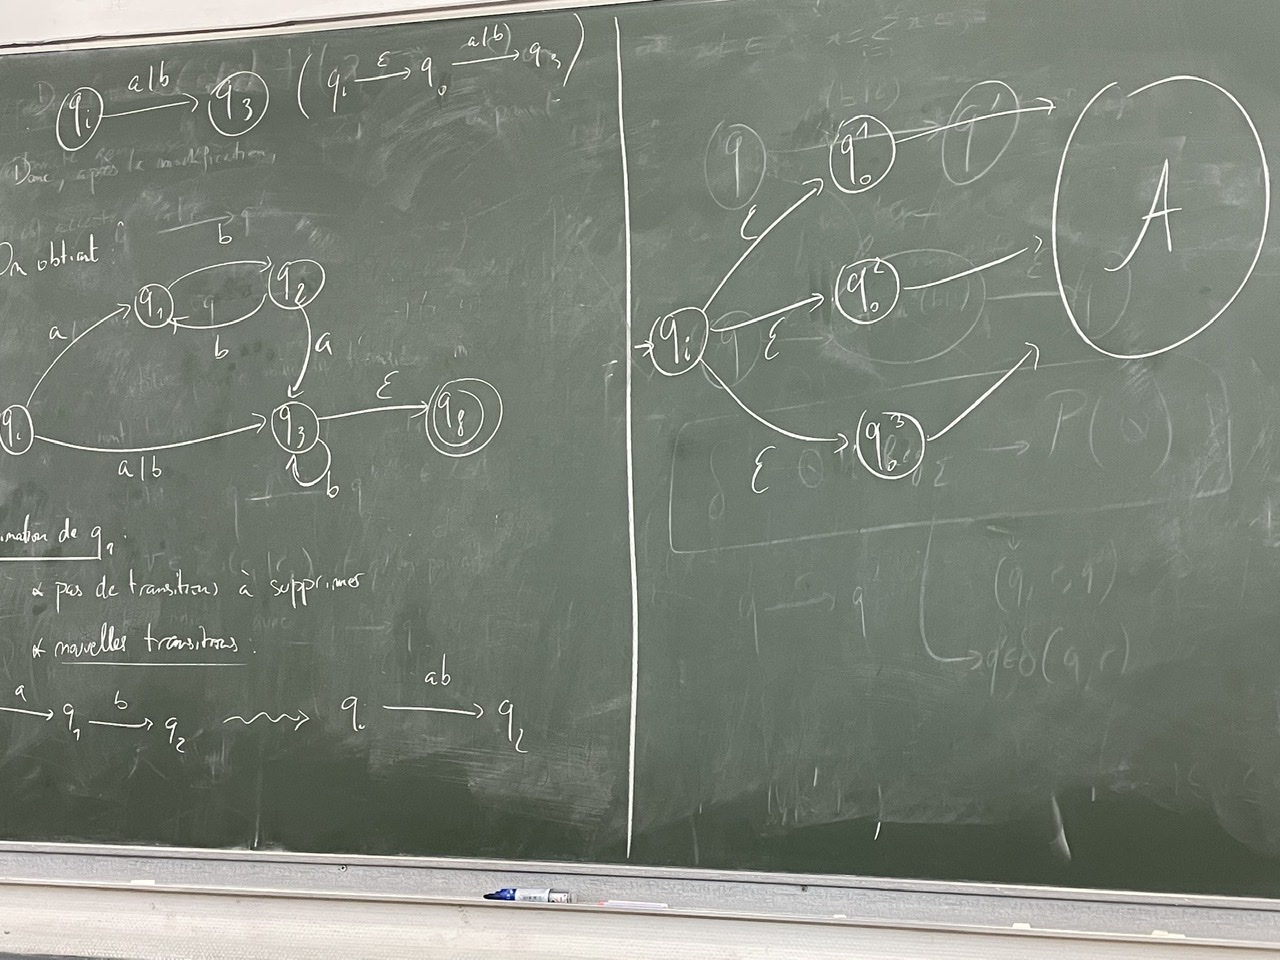
\includegraphics[scale=0.2]{Dessin/Tableau2.jpeg}
        %vive le premium qui donne 4min de temps de compilation 
        \vspace{2cm}
        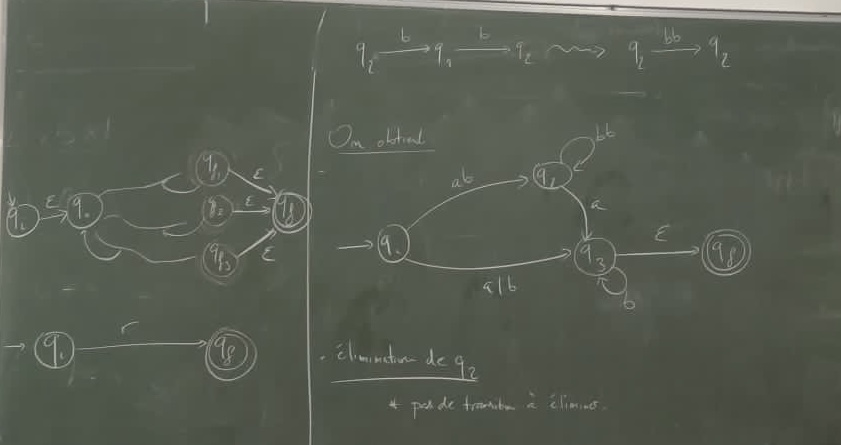
\includegraphics[scale=0.2]{Dessin/Tableau3.jpeg}
        \vspace{2cm}
        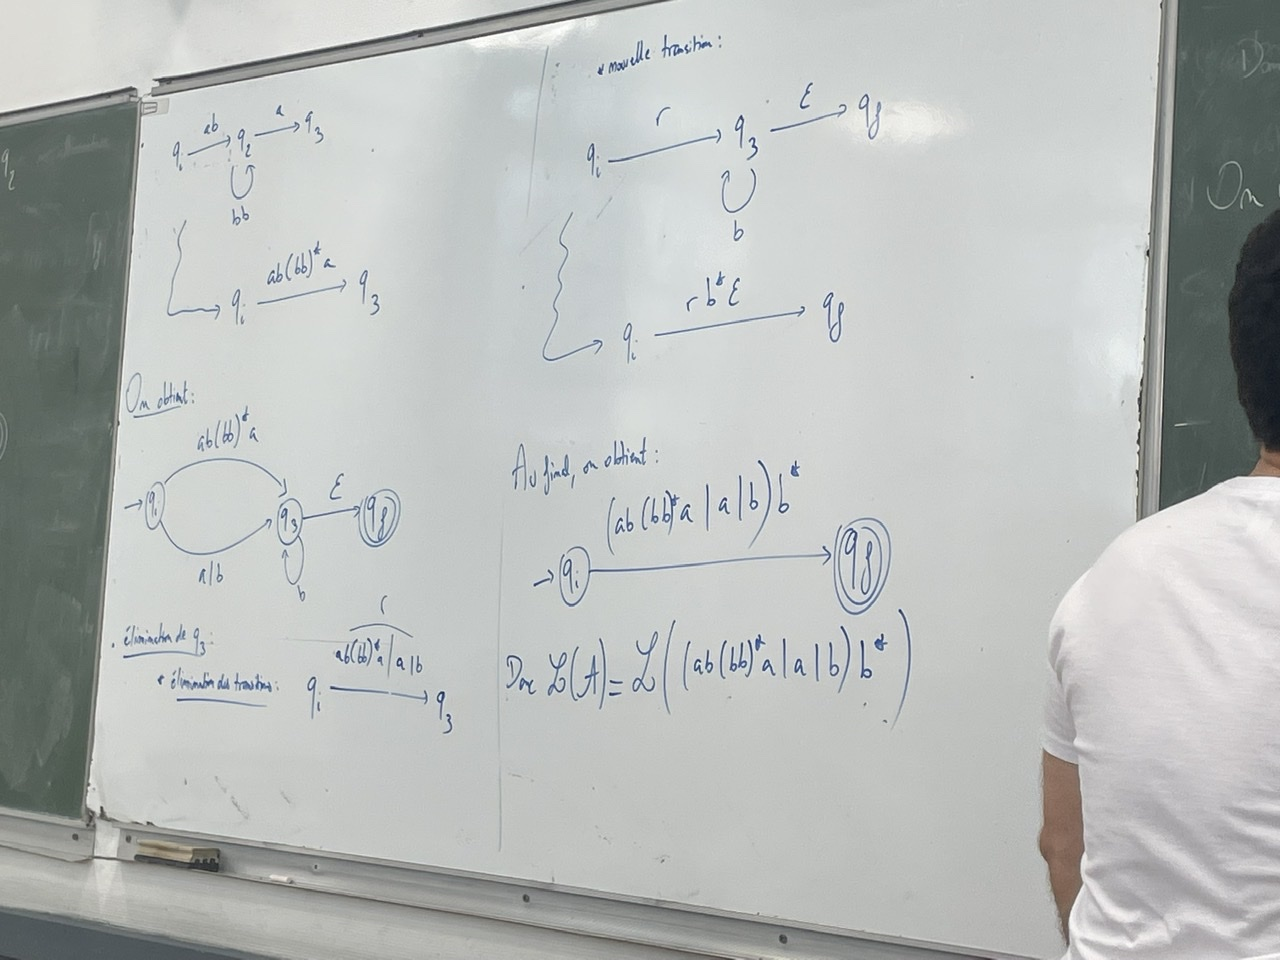
\includegraphics[scale=0.2]{Dessin/Tableau4.jpeg}
        
        
    \end{example}
    
    On remarquera les points suivants :
    %
    \begin{enumerate}
        \itt L'expression obtenue peut varier selon l'ordre dans lequel on traite les états.
        
        \itt L'expression obtenue peut être de taille exponentielle en le nombre d'états de $\bcA$.
    \end{enumerate}
    
    \subsection{Propriétés des langages reguliers}
    
    \subsubsection{Stabilité par opérations ensemblistes et miroir}
    
        Une fois le lien etabli entre les language regulier et automates on peut montrer facilement certiane propriete des language regulier 
        
    \begin{theorem}{Stabilité par complémentaire}{}
        Soit $L \in \Reg_\Sigma$. Alors $\overline{L} \in \Reg_\Sigma$.
    \end{theorem}
    
    \begin{nproof}
        Soit $A = \p{Q, \Sigma, q_0, F, \delta}$ tel que $\bcL\p{\bcA} = L$
        Posons $A' =  \p{Q, \Sigma, q_0, Q \backslash F, \delta}$
        
        Soit $v \in \Sigma^\star$. Comme $A$ est déterministe et complet, il existe un unique chemin $q_0 \lima{v}_A^\star q$.
    
        Ce chemin est également l'unique chemin dans $A'$ depuis $q_0$ pour $v$. On a alors :
        %
        \begin{align*}
                && v &\in L : \bcL\p{\bcA}\\
            \iff && q &\in F\\
            \iff && q &\not\in Q \backslash F\\
            \iff && v &\not\in \bcL\p{\bcA'}
        \end{align*}
        Donc $\bcL\p{\bcA'} = \overline{L}$
    
    \end{nproof}
    
    \begin{corollary}{}{}
        Soient $\p{L_1, L_2} \in \p{\Reg_\Sigma}^2$. Alors $L_1 \backslash L_2 \in \Reg_\Sigma$.
    \end{corollary}
        
    \begin{nproof}
        $L_1 \backslash L_2 = L_1 \cup \overline{L_2 \in Reg_\Sigma}$
    \end{nproof}
    
    \begin{theorem}{Stabilité par mirroir}{}
        Soit $L \in Reg_\Sigma$.
        Alors $L^R \in Reg_\Sigma$ avec $L^R \in \Reg_\Sigma$ le langage miroir de $L$.
    \end{theorem}
    
    \begin{nproof}
        Soit $\bcA = \p{Q, \Sigma, I, F, \delta}$ un NFA tel que $L = \bcL\p{\bcA}$.
        
        On pose $\bcA' = \p{Q, \Sigma, I', F', \delta'}$ avec :
        %
        \begin{enumerate}
            \itt $I' = F$
            \itt $F' = I$
            \itt $q_1 \lima{a}_\bcA q_2 \in \delta \iff q_2 \lima{a}_{\bcA'} q_1 \in \delta'$
        \end{enumerate}
        %
        Montrons que $\bcL\p{\bcA'} = L^R$. Soit $v \in \Sigma^\star$, on a :
        %
        \begin{enumerate}
            \itt si $v = \epsilon$ : $\epsilon \in L^R \iff \epsilon \in L \iff I \cap F \neq \emptyset \iff F' \cap I' \neq \emptyset \iff \epsilon \in \bcL\p{\bcA'}$
            
            \itt sinon : $v = a_1 \dots a_n$.
            Alors $v \in L^R \iff a_n \dots a_1 \in L \iff q_n \lima{a_{n}}{}_\bcA q_{n-1} \lima{a_{n-1}}{}_\bcA \dots \lima{a_1}{}_\bcA q_0$ avec $q_n \in I$ et $q_0 \in F \iff q_0 \lima{a_1}{}_{A'} q_1 \lima{a_2}{}_{A'} q_2 \dots \lima{a_n}{}_{A'} q_n$ avec $q_0 \in I'$ et $q_n \in F' \iff v \in \bcL\p{\bcA'}$
        \end{enumerate}
    \end{nproof}
    
    \subsubsection{Lemme de l'étoile}
    
    Nous allons maintenant nous intéresser à la question suivante :
    Soit $\Sigma$ un alphabet, soit $L \subseteq \Sigma^\star$. $L$ est-il régulier ?
    \begin{enumerate}
        \itt Si on trouve une expression régulière ou un automate dont le langage est $L$, alors la réponse est oui $\dots$
        \itt Si on en trouve pas
        \begin{enumerate}
            \itt soit la réponse est non
            \itt soit on a "pas assez cherché"
        \end{enumerate}
    \end{enumerate}
    Si on pense que la réponse est non, comment prouver qu'un langage n'est pas régulier ?
    
    \begin{example}{}{}
        $\Sigma = \ens{a, b}$
        \begin{enumerate}
            \itt $L_1 = \ens{a^n b^n\enstq n \equiv m \intc{2}}$
            $L_1 = \p{a^2}^\star \p{b^2}^\star \vert \p{a^2}^\star a \p{b^2}^\star b$
            donc $L_1 \in Reg_\Sigma$
            \itt $L_2 = \ens{a^n b^n \enstq n \in \bcN}$
            On va voir maintenant que $L_2 \notin Reg_\Sigma$
        \end{enumerate}
    \end{example}
    
    Voici un critère appelé lemme de l'étoile (ou pumping lemma en anglais), qui permet de montrer qu'un certain nombre de langages ne sont pas réguliers.
    
    \begin{theorem}{Lemme de l'étoile}{}
        Soit $\Sigma$ un alphabet. Soit $L \in Reg_\Sigma$
        Alors : $\exists n \in \bcN^\star$ tel que
      $\forall u \in L$ tel que $\mod{u} \geq n$,
        $\exists \p{x, y, z} \in \p{\Sigma^\star}^3$ tels que :
        \begin{enumerate}
            \itt $u = x y z$
            \itt $y \neq \epsilon$
            \itt $\mod{xy} \leq n$
            \itt $x y^\star z \subseteq L$
        \end{enumerate}
    \end{theorem}
    
    \begin{nproof}
        Soit $\bcA = \p{Q, \Sigma, q_0, F, \delta}$ tel que $L = \bcL\p{\bcA}$
        Posons $n = \mod{Q}$.
        Soit $u \in L$ tel que $\mod{u} \geq n$ : $u = q_1 \dots q_n$ avec $m \geq n$.
        Comme $u \in \bcL\p{\bcA}$, il existe un chemin :
        $q_0 \lima{a_1}{}_\bcA q_1 \lima{a_2}{}_\bcA q_2 \dots \lima{a_m}{}_\bcA q_m$ avec $q_m \in F$.
        On passe par $m=1$ états de $Q$, et $\mod{Q} = n \leq m < n + 1$.
        Donc par principe des tirroirs de Diridlet :
        $\exists i \neq j$ tels que $q_i = q_j$
        Choisissons $i$ et $j$ les plus petits possibles. On a donc un cycle de taille $j-i$ dans ce chemin. En posant
        \begin{enumerate}
            \itt $x = a_0 \dots a_{i-1}$
            \itt $y = a_i \dots a_{j-1}$
            \itt $z = a_j \dots a_m$
        \end{enumerate}
        on a
        \begin{enumerate}
            \itt $u = x y z$
            \itt $y \neq \epsilon$ (car $i<j$)
            \itt $\mod{xy} \leq n$ car $i$ et $j$ ont été choisis les plus petits possibles, donc tous les $q_k$ pour $k \in \iint{0, j - 1}$ sont distincs 2 à 2, donc $j \leq n = \mod{Q}$
        \end{enumerate}
        On a donc un chemin ;
        $q_0  \lima{x}{}_\bcA^\star q_i = q_j \lima{z}{}^\star q_n \in F$
        %boucle en dessous du qi = qj
        Donc $\forall k \in \bcN, q_0 \lima{x y^k z}{}_\bca^\star q_m \in F$
        ie $xy^kz \in \bcL\p{\bcA} = L$
        donc $xy^kz \subseteq L$
    \end{nproof}
    On remarque que en général, on utilise le terme de l'étoile de la manière suivante :
    \begin{enumerate}
        \item On veut montrer qu'un langage $L \subseteq \Sigma^\star$ n'est pas régulier
        \item Par l'absurde, on suppose que $L$ est régulier
        \item D'après le lemme de l'étoile, $\exists n \in \bcN^\star$ tel que ...
        \item On choisis "intelligemment" un $u \in L$ tel que $\mod{u} \leq n$
        \item On montre que, \emph{pour tout} découpage possible $u = x y z$ avec $\mod{xy} \leq n$ et $y \neq \epsilon$ on a pas $x y^\star z \subseteq L$ : absurde.
        \item donc $L$ n'est pas régulier
    \end{enumerate}
    
    \begin{theorem}{}{}
        Le langage $L = \ens{a^n b^n \enstq n \in \bdN}$ n'est pas régulier.
    \end{theorem}
    
    \begin{nproof}
        Par l'absurde, on suppose que $L$ est régulier. D'après le lemme de l'étoile : $\exists n \in \bcN^\star$ tel que $\mod{u} \geq n$...
        Considérons $u = a^n b^n$
        Soit $u = x y z$ tel que $y \neq \epsilon$ et $\mod{xy} \leq n$
        Donc $\exists  \p{i, j} \in \bcN^2$ tel que
        \begin{enumerate}
            \itt $x = a^i$
            \itt $y =a^j \p{j > 0}$
            \itt $z = a^{n-i-j} b^n$
        \end{enumerate}
        et $x y^\star z \subseteq L$
        ie $\forall x \in \bcN \quad a y^\star z \in L$ en particulier $x y^0 z \in L$
        Donc $a^{n-j} b^n \in L$
        avec $j>0$ \emph{absurde} car $n-j neq n$
        donc $L$ n'est pas régulier
    \end{nproof}
    
    \begin{warning}{}{}
        Il ne faut pas s'embrouiller sur la manière dont les quantificateurs alternent : si on prend la contraposée du lemme de l'étoile, on a :
        %
        Si $\forall n \in \bdN^\star$, $\exists u \in L$ tel que $\mod{u} \geq ,$
        
        et $\forall \p{x, y, z} \in \Sigma^\star$ tel que $u = xyz$, $y \neq \epsilon$, $\mod{xy} \leq n$ et $\exists k \in \bdN$ tel que $xy^kz \not\in L$
        
        alors $L$ n'est pas régulier.
        
        Autrement dit :
        %
        \begin{enumerate}
            \itt On ne choisit pas le $n$ ;
            \itt on peut ensuite choisir $u$ comme o veut en fonction de $n$, parmi les $u \in L$ tel que $\mod{u} \geq n$
            
            \itt On doit considérer \bf{tous} les découpages possibles :
            %
            $u = xyz$ avec $\mod{xy} \leq n$ et $y \neq \epsilon$.
            
            Ainsi il vaut mieux \guill{bien choisir} $u$ pour que tous les découpages possibles se ressemblent. 
            
            \itt On peut choisir $k$ comme on veut pour que $xy^kz \not\in L$.
        \end{enumerate}
    \end{warning}
    
    Parfois, pour montrer qu'un langage $L$ n'est pas régulier, il est plus facile de raisonner sur un autre langage $L'$ dépendant de $L$, tel que $L \in \Reg_\Sigma \implies L' \in \Reg_\Sigma$.
    
    On montre alors, en vertu du lemme de l'étoile, que $L'$ n'est pas régulier et donc que $L$ n'est pas régulier.
    %
    \begin{example}{}{}
        On considère $\hg{L = \ens{a^nb^n \enstq n \neq m}}$.
        
        Si $L$ était régulier, alors $a^\star b^\star \backslash L$ serait régulier. Or :
        %
        \[ a^\star b^\star \backslash L = \ens{a^nb^n \enstq n = m} = \ens{a^nb^n \enstq n \in \bdN}\]
        %
        n'est pas régulier d'après le théorème précédent.
    \end{example}
    
    Les langages réguliers (et les automates) sont donc très utiles pour chercher des motifs simples dans un texte. On souhaiterait s'en servir pour effectuer une analyse syntaxique du code source d'un programme. Par exemple, trouver tous les mots clés (\texttt{while}, \texttt{for}, \texttt{if}, \texttt{float}, \texttt{float}, \dots) du langage de programmation dans le code source est faisable à l'aide d'un automate. Mais qu'en est-il d'autres propriétés à vérifier ? Par exemple, peut-on vérifier si les expressions présentes dans le code source sont bien parenthésées ?
    
    Pour étudier ce problème, étudions l'exercice suivant :
    %
    \begin{exercise}{}{}
        $\Sigma = \ens{(, ), [, ], \{, \}, <, >}$
        %
        $L = \ens{u \in \Sigma^\star \enstq u \ \text{est bien parenthésé}}$ est-il régulier ?
        %
        \tcblower
        %
        Par l'absurde, supposons que $L$ est  régulier. D'après le lemme de l'étoile, on a :
        %
        \[\exists n \geq 0, \forall u \in \Sigma^\star, \mod{u} \geq n \implies \exists x, y, z \in \Sigma^\star \ \text{tel que} \ \left\lbrace\begin{array}{l}
            xyz = u\\
            y \neq \epsilon\\
            y^\star \in L\\
            \mod{xy} \leq n\\
        \end{array}\right.\]
        Soit $n \geq 0$, soit $u = (^n )^n$,
        %
        Alors on a $u \in L$ ainsi que $\mod{u} \geq n$
        Mais soient $x, y, z \in \Sigma^\star$ tel que
        $\left\lbrace\begin{array}{l}
            xyz = u\\
            y \neq \epsilon\\
            xy^\star z \in L\\
            \mod{xy} \leq n\\
        \end{array}\right.$
        Alors $\mod{xy} \leq n \implies xy = (^{\mod{xy}} \implies y = (^{\mod{y}}$
        $xyz \in L \implies xy(^{\mod{y}}z \not\in L \implies xy^2z \notin L$ : Absurde !
        
    \end{exercise}
    
    La classe des langages réguliers est donc trop restreinte
    
    on va maintenant en étudier une autre.
    
    \section{Grammaires non contextuelles}
        
    \subsection{Grammaires et langages non contextuels}
    
    \begin{definition}{Grammaire non contextuelle}{}
        On appelle \hg{grammaire non contextuel} (\hg{context-free grammar} en anglais) la donnée d'un \hg{quadruplet $\bcG = \p{\bcV, \Sigma, \bcR, S}$} où :
        %
        \begin{enumerate}
            \itast \hg{$\bcV$} est un \hg{alphabet} de \hg{symboles} appelés \hg{non terminaux} (on parle aussi de \hg{variables}).
        
            \itast \hg{$\Sigma$} est un \hg{alphabet} de \hg{symboles} appelés \hg{terminaux}, et est tel que \hg{$\Sigma \cap \bcV = \emptyset$}.
            
            \itast \hg{$\bcR \subset \bcV \times \p{\Sigma \sqcup \bcV}^\star$} est un \hg{ensemble fini} de \hg{règles de production}.
            
            \itast \hg{$S \in \bcV$} est un \hg{symbole non terminal} appelé \hg{symbole initial} (ou \hg{axiome}) \hg{de la grammaire}.
        \end{enumerate}
    \end{definition}
    
    \begin{notation}
        \begin{enumerate}
            \itt On désigne généralement un \hg{symbole non terminal} de \hg{$\bcV$} par une \hg{lettre majuscule} comme \hg{$S$}, \hg{$T$}, \hg{$U$}, \hg{$\dots$}.
            
            \itt On désigne généralement un \hg{symbole terminal} de \hg{$\Sigma$} par une \hg{lettre minuscule} comme \hg{$a$}, \hg{$b$}, \hg{$c$}, \hg{$\dots$}.
            
            \itt On désigne généralement une \hg{règle de production} de la forme \hg{$\p{T, \bcu} \in \bcR$} par la notation \hg{$T \rightarrow \bcu \in \bcR$}.
            
            \itt Si \hg{$n \in \bdN$ règles} ont le \hg{même symbole} à gauche, donc de forme \hg{$T \rightarrow u_1 \in \bcR$}, \hg{$T \rightarrow u_2$}, \hg{\dots}, $\hg{T \rightarrow u_n}$, on désignera cet \hg{ensemble de règle} par \hg{$T \rightarrow v_1 \vert v_2 \vert \dots \vert v_n$}.
        \end{enumerate}
    \end{notation}
    
    On fera les remarques suivantes :
    %
    \begin{enumerate}
        \itt Une règle peut parfaitement être vide à droite : $T \to \epsilon$.
        
        \itt Le terme de \emph{grammaires non contextuelles} vient du fait qu'on n'a pas de règle de la forme $aTb \to v$. Si on autorise ce genre de règles, on parle d'ailleurs de \emph{grammaires contextuelles}, mais ce type de grammaire n'est pas au programme de la \textsf{MPI}.
        
        \itt Les \emph{grammaires non contextuelles} sont aussi appelées \emph{grammaires hors contexte} ou \emph{grammaire algébriques}.
    \end{enumerate} 
    
    Puisque les \emph{grammaires non contextuelles} sont le seul type de grammaire au programme, on les appellera simplement \emph{grammaires}.
    
    \begin{definition}{Dérivation immédiate}{}
        Soient \hg{$\bcG = \p{\bcV, \Sigma, \bcR, S}$} une \hg{grammaire}, \hg{$u = u_1Xu_2 \in \p{\Sigma \cup \bcV}^\star \bcV \p{\Sigma \cup \bcV}^\star$} et \hg{$v \in \p{\Sigma \cup \bcV}^\star$}. On dit que \hg{$u$ se dérive immédiatement en $v$}, et on note \hg{$u \Rightarrow v$}, s'il existe \hg{$r \in \p{\Sigma \cup \bcV}^\star$} tel que :
        %
        %
        \[ \hg{X \rightarrow r \in R} \qquad\qquad\et\qquad\qquad \hg{v = u_1 r u_2}\]
        %
        De plus, on dit que c'est une \hg{dérivation immédiate à gauche} \emph{(resp. \hg{à droite})} si \hg{$u_1 \in \Sigma^\star$} \emph{(resp. si \hg{$u_2 \in \Sigma^\star$})}.
    \end{definition}
    
    \begin{definition}{Dérivation}{}
        On note $\Rightarrow^\star$ la clôture réflexive et transitive de $\Rightarrow$. Si $u \Rightarrow^\star v$, on dit que \hg{$u$ se dérive en $v$}.
        
        Une suite de dérivations immédiates $u_1 \Rightarrow \dots \Rightarrow u_n$ est appelé une \hg{dérivation}.
        Une dérivation est \hg{à gauche} \emph{(resp. \hg{à droite})} lorsque \hg{toutes les dérivations qui la composent sont à gauche} \hg{(resp. \hg{à droite})}.
    \end{definition}
    
    \begin{definition}{Langage engendré par une grammaire}{}
        Soit \hg{$\bcG = \p{\bcV, \Sigma, \bcR, S}$} une \hg{grammaire}. On appelle \hg{langage engendré par $\bcG$} le langage 
        %
        \[ \hg{\bcL\p{\bcG} = \ens{v \in \Sigma^\star \enstq S \Rightarrow^\star v }}\]
        Un langage engendré par une grammaire non contextuelle est appelé \hg{langage non contextuel}.
    \end{definition}
    %
    \begin{notation}
        On note \hg{$\CFL_\Sigma$} (context free language) l'\hg{ensemble des langages non contextuels sur $\Sigma$}.  
    \end{notation}
    
    \begin{example}{Langages de Dyck}{}
        On prend \hg{$\Sigma = \ens{(,) ,\{,\} ,[,] ,<,>}$} et le \hg{langage de \textsc{Dyck} $\bsL = \ens{v \in \Sigma^\star \enstq v \ \text{est bien parenthésé}}$}.\medskip
        
        On considère \hg{$\bcG = \p{\bcV, \Sigma, \bcR, S}$} avec \hg{$\bcV = \ens{S}$} et les règles \hg{$\hg{S \to \p{S}S \mid \epsilon \mid \intc{S} S \mid \ens{S} S \mid <S> S}$}.
        
        On a par exemple :
        %
        \[ \hg{S \Rightarrow \p{S} S \Rightarrow \p{\p{S} S} S \Rightarrow \p{\p{\p{S} S} S} S \Rightarrow \p{\p{\p{S} S} S} \p{S} S \Rightarrow \p{\p{\p{S} S} S} \p{\p{S} S} S \Rightarrow^\star \p{\p{\p{}}} \p{\p{}}}\]
        %
        Généralement, on retrouve \hg{$\bsL = \bcL\p{G}$}.
    \end{example}
    
    \begin{example}{Formules propositionelles}{}
        On a $\bcG_\text{prop} : \Sigma = \ens{a, b, c} \cup \ens{\neg, \lor, \land \rightarrow, (, )}$, $\bcV = \ens{S}$, et 
        %
        \[ \bcR = S \rightarrow a \mid b \mid c \mid \dots \mid \p{S} \mid \neg S \mid \neg S \lor S \mid S \land S \mid S \rightarrow S\]
        %
        $\bcL\p{\bcG_\text{prop}} = \ens{\text{formules propositionelles syntaxiquement correctes dont les variables sont} \ a, b, c, \dots}$.\medskip
        
        Par exemple, pour générer $S \Rightarrow^\star \p{a \lor \neg \p{b \land c}} \rightarrow a$, on a :
        %
        \begin{align*}
            S &\Rightarrow S \rightarrow \hg S\\
            &\Rightarrow \hg S \rightarrow a\\
            &\Rightarrow \p{\hg S} \rightarrow a\\
            &\Rightarrow \p{S \lor \hg S} \rightarrow a\\
            &\Rightarrow \p{S \lor \neg \hg S} \rightarrow a\\
            &\Rightarrow \p{S \lor \neg \p{\hg S}} \rightarrow a\\
            &\Rightarrow \p{S \lor \neg \p{S \land \hg S}} \rightarrow a\\
            &\Rightarrow \p{S \lor \neg \p{\hg S \land c}} \rightarrow a\\
            &\Rightarrow \p{\hg S \lor \neg \p{b \land c}} \rightarrow a\\
            &\Rightarrow \p{a \lor \neg \p{b \land c}} \rightarrow a
        \end{align*}
    \end{example}
    
    
    \begin{example}{Formules du premier ordre}{}
        $\bcG_\text{FO} : \Sigma = \Sigma_\bcV \cup \Sigma_\bcF \cup \Sigma_\bcR \cup \Sigma_\bcC \cup \ens{\neg, \lor, \land, \rightarrow, \exists, \forall, (, )} \cup \ens{,}$ où :
        %
        \begin{enumerate}
            \itt $\Sigma_\bcV = \ens{x, y, z, \dots}$ (variables du premier ordre) ;
            \itt $\Sigma_\bcF = \ens{f \p{1}, g\p{2}, h\p{3}, \dots}$ (symboles de fonctions) ;
            \itt $\Sigma_\bcR = \ens{= \p{2}, \leq \p{2}, \asymp \p{2}, \equiv \p{2}, \dots}$ (symboles de relations) ;
            \itt $\Sigma_\bcC = \ens{a, b, c, \dots}$ (symboles de constantes).
        \end{enumerate}
        %
        On a également $\bcV = \ens{S, T, A, V, F}$ de sorte qu'on ait les règles de production suivantes :
        %
        \begin{enumerate}
            \itt $S \rightarrow F$ ;
            
            \itt $F \rightarrow A \mid \neg F \mid F \land F \mid F \rightarrow F \mid \p{F} \mid \exists V, F \mid \forall V, F$ ;
            
            \itt $V \rightarrow x \mid y \mid z \mid \dots$ (avec $\Sigma_\bcV$) ;
            
            \itt $A \rightarrow T = T \mid T \leq T \mid T \asymp T \mid T \equiv T \mid \dots$ (avec $\Sigma_\bcR$) ;
            
            \itt $T \rightarrow a \mid \b \mid c \mid \dots$ (avec $\Sigma\bcC$)
            
            \itt $T \rightarrow f\p{T} \mid g\p{T, T} \mid k\p{T, T, T} \mid \dots$ (avec $\Sigma_\bcF$)
        \end{enumerate}
        %
        Dès lors, $\bcL\p{\bcG_\text{FO}} = \ens{\text{formules du premier ordre syntaxiquement correctes}}$.
    \end{example}

    \begin{example}{Mini-langage}{}
        Soit \hg{$\bcG = \p{\bcV, \Sigma, \bcR, S}$} la \hg{grammaire non contextuelle} telle que :
        %
        \begin{enumerate}
            \itt L'alphabet des symboles non terminaux est \hg{$\bcV = \ens{S, I, E, V, N, C}$}.
            
            \itt L'alphabet des symboles terminaux est \hg{$\Sigma = \ens{\texttt{x}, \texttt{y}, \texttt{print}, \texttt 0, \texttt 1, \texttt 2, \dots, \texttt 9, \texttt =, \texttt +, \texttt ; , \texttt (, \texttt ), \epsilon}$}.
            
            \itt Les règles de production sont \hg{$\bcR = \begin{array}[t]{rcl}
                S &\rightarrow & I\texttt{;}S \mid \epsilon  \\
                I &\rightarrow & V\texttt{ = }E \mid \texttt{print(E)} \\
                E &\rightarrow& E + E \mid N \mid V\\
                V &\rightarrow& x \mid y\\
                N &\rightarrow& CN \mid C\\
                C &\rightarrow & \texttt 0 \mid \texttt 1 \mid \texttt 2 \mid \dots \mid \texttt 9
            \end{array}$}
        \end{enumerate}
        %
        Le langage \hg{$\bcL\p{\bcG}$} engendré par une telle grammaire est appelé \hg{mini-langage}. On y obtient par exemple l'expression \hg{$\texttt{x = 42;} \in \bcL\p{\bcG}$} avec la dérivation suivante :
        %
        \begin{align*}
            S &\Rightarrow \hg I\texttt{;}S\\
            &\Rightarrow \hg V\texttt{ = }E\texttt{;}S\\
            &\Rightarrow \texttt{x = }\hg E\texttt{;}S\\
            &\Rightarrow \texttt{x = }\hg N\texttt{;}S\\
            &\Rightarrow \texttt{x = }\hg CN\texttt{;}S\\
            &\Rightarrow \texttt{x = 4}\hg N\texttt{;}S\\
            &\Rightarrow \texttt{x = 4}\hg C\texttt{;}S\\
            &\Rightarrow \texttt{x = 42;}\hg S\\
            &\Rightarrow \texttt{x = 42;}
        \end{align*}
    \end{example}
    
    
    
    \begin{theorem}{Non contextualité des langages réguliers}{}
        Soit $\Sigma$ un alphabet.
        $\Reg_\Sigma \subseteq \CFL_\Sigma$.
        De plus, si $\mod{\Sigma} \geq 2$, l'inclusion est stricte. %la preuve svp
    \end{theorem}
    \begin{nproof}
        On montre d'abords l'inclusion
        Soit $L \subseteq Reg_\Sigma$
        Il existe un automates $\bcA = (Q,\Sigma, q_0, F, \sigma)$ tel que $L= \bsL(A)$
        on choisit $\bcA$ un CDFA.
        
        On construit $\bcG_\bcA = \p{\mu, \Sigma, \bcR, X_{q_0}}$
        Avec $\mu = \ens{X_q \enstq q \in Q}$
        et 
        \begin{enumerate}
            \itt $\bcR X_q \to q X_q$ pour tout $\p{q, a, q'}$ tel que $\lima{a}{}_\bcA q'$
            \itt $X_q \to \epsilon$ pour tout $q \in F$
        \end{enumerate}
        Montrons que $X_q \Rightarrow^\star vX_{q'}$ ssi $q \lima{v}{}_\bcA^\star q'$
        Par récurrence sur $\mod{v}$ :
        \begin{enumerate}
            \itt $\mod{v} = 0 v = \epsilon$ on a bien $X_q \Rightarrow^\star X_q$ et $q \lima{\epsilon}{}_\bcA^\star q$ quelque soit les grammaires et les automates considérés.
            De plus, comme $\bcA$ n'a pas d'$\epsilon$-transition, il n'y a pas d'autre chemin possible pour lire $\epsilon$ (i.e. $q \lima{\epsilon}{}\bcA^\star q' avec q \neq q'$)
            Et par construction de $\bcG_\bcA$, il n'y a pas d'autres dérivation possible $X_q \Rightarrow^\star X_{q'} avec q \neq q'$
            \itt $\mod{v} > 0$ : Supposons la propriété vraie pour les mots de taille $n$. Montrons qu'elle est vraie pour les mots $v$ de taille $n + 1$.
            On pose $v = ua$ avec $\mod{u} = n$.
            Par (HR) $X_q \Rightarrow^\star u X_{q'}$ ssi $q \lima{u}{}_\bcA^\star q'$
            L'automate $\bcA$ étant complet et déterministe : $\exists q^n \in Q$ tel que $q' \lima q''$
            Par construction de $\bcG_\bcA$, on a : $X_{q'} \to aX_{q''}$
            Ainsi : $X_q \Rightarrow^\star u X_{q'} \Rightarrow uaX_{q''}$
            Réciproquement, si $X_q \Rightarrow^\star uaX_{q''}$ alors, forcément, la dernière étape est de la forme : $X_q \Rightarrow^\star uX_{q'} \Rightarrow uaX_{q''}$
            En effet, pour cette grammaire $\bcG_\bcA$, on peutfacilement montrer que si un mot est dérivable dans $\bcG_\bcA$ depuis une variable $X_q$, alors
            \begin{enumerate}
                \itt soit ce mot ne contient pas de variable
                \itt soit il possède une unique variable à la fin.
            \end{enumerate}
            Donc, la dernière règle utilisée est de la forme $X_{q'} \to aX_{q''}$ donc $q' \lima{q}{}_\bcA q'' $
            De plus, par (HR) $q \lima{u}{}_\bcA^\star q'$ Ainsi : $q \lima{v}{}\bcA^\star q''$
        \end{enumerate}
        Finalement :
        $v \in L$
        \begin{align*}
            v \in L &\iff q_0 \lima{v}^\star q \in F\\
            &\iff X_{q_0} \Rightarrow^\star v X_q \text{avec} q \in F\\
            &\iff X_{q_0} \Rightarrow^\star v \ \text{car le seul moyen de faire disparaître} \ X_q \ \text{est d'utiliser} \ X_q \to \epsilon \ \text{quand} \ q \in F\\
            &\iff v \in \bcL\p{\bcG_\bcA}
        \end{align*}
        
        Si $\mod{\Sigma} \geq 2$, montrons que l'inclusion est stricte. Soient $\p{a, b} \in \Sigma^2$ tels que $a \neq b$. On a montré, l'aide du \emph{lemme de l'étoile}, que $\ens{a^nb^n,\ n \in \bdN} \not\in \Reg_\Sigma$. Montrons que $\ens{a^nb^n,\ n \in \bdN} \in \CFL_\Sigma$. Soit $\bcG$ la grammaire telle que :
        %
        \begin{enumerate}
            \itt $\bcV = \ens{S}$
            \itt $\bcR = S \rightarrow aSb \mid \epsilon$
        \end{enumerate}
        %
        Montrons par récurrence sur $n \in \bdN$ que $a^nb^n \in \bcL\p{\bcG}$ :
        %
        \begin{enumerate}
            \itt Pour $n = 0$, $S \Rightarrow \epsilon$, et $\epsilon = a^0b^0 \in \bcL\p{\bcG}$.
            
            \itt Supposons que $S \rightarrow^\star a^nb^n$. On a $S \Rightarrow aSb \Rightarrow aa^nb^nb \Rightarrow a^{n+1}b^{n+1}$, d'où $a^{n+1}b^{n+1} \in \bcL\p{\bcG}$.
        \end{enumerate}
        %
        De plus, il est facile de remarquer que ce sont les seuls mots qu'il est possible de générer avec cette grammaire. En effet, tout mot généré depuis $S$ contient le même nombre de $a$ et de $b$, et n'a d'abord que des $a$, puis que des $b$. Ainsi $\ens{a^nb^n,\ n \in \bdN} = \bcL\p{\bcG} \in \CFL_\Sigma$.
    \end{nproof}
    
    \subsection{Ambiguïté d'une grammaire}
    
    Les dérivations telles que nous les avons définies, ne font pas apparaître clairement ce qu'il se passe lorsqu'on engendre un mot à l'aide d'une grammaire, \ie le processus par lequel le mot est obtenu.
    Pour obtenir cette information, il nous faut avoir recours à une structure plus complexe. On remarque déjà que le processus par lequel on obtenait un mot à l'aide de dérivation successives, opère en modifiant progressivement une expression. Il serait donc utile d'utiliser une structure arborescente pour représenter les dérivations :
    
    \begin{definition}{Arbre de dérivation}{}
        Soit \hg{$\bcG = \ens{\bcV, \Sigma, \bcR, S}$} une \hg{grammaire non contextuelle}. On appelle \hg{arbre de dérivation} un \hg{arbre} étiqueté tel que :
        %
        \begin{enumerate}
            \itast la \hg{racine} est étiquetée par \hg{$S$} ;
            
            \itast tout \hg{n\oe{}ud interne} est étiqueté par un \hg{symbole de $\bcV$} ;
            
            \itast Toute \hg{feuille} est étiquetée par un \hg{symbole de $\Sigma \cup \ens{\epsilon}$} ;
            
            \itast Si \hg{$u_1, \dots u_n$} sont les \hg{fils d'un n\oe{}ud} étiqueté \hg{$X$}, alors il existe une \hg{règle $X \rightarrow u_1 \dots u_n \in \bcR$}.
        \end{enumerate}
        %
        Un \hg{arbre de dérivation} dont \hg{les feuilles concaténées de gauche à droite forment un mot $u$} est appelé \hg{arbre de dérivation de $u$}, \hg{arbre syntaxique de $u$} ou encore \hg{arbre de dérivation syntaxique de $u$}.
    \end{definition}
    %
    Pour un mot donné, il n'y a pas unicité (pas plus que pour les dérivations) de l'arbre de dérivation de ce mot. syntaxe On illustre ces notions ci-dessous :
    %
    \begin{example}{Arbre de dérivation syntaxique}{gramambi}
        On considère \hg{$\bcG_\text{arithm} = \p{\bcV, \Sigma, \bcR, S}$} la \hg{grammaire non contextuelle} telle que :
        %
        \begin{enumerate}
            \itt L'alphabet des symboles non terminaux est \hg{$\bcV = \ens{S, E}$}
            
            \itt L'alphabet des symboles terminaux est \hg{$\Sigma = \ens{0, 1, 2,\dots, 9, +, -, \times, (, )}$}
            %
            \itt Les règles de productions sont $\hg{\bcR = \begin{array}[t]{rcl}
                E &\rightarrow& E  \\
                E &\rightarrow& E + E \mid E - E \mid E \times E \mid \p{E}\\
                E &\rightarrow& 0 \mid 1 \mid 2 \mid \dots \mid 9
            \end{array}}$
        \end{enumerate}
        %
        On donne ci-dessous deux arbres de dérivation de  \hg{$2+4\times 3 - 7 \in \bcL\p{\bcG_\text{arithm}}$} :\newline
        
        \begin{minipage}{0.5\linewidth}
        \begin{center}
            \begin{tikzpicture}[nodes={}, ->,
                level 2/.style = {sibling distance = 2.5cm},
                level 3/.style = {sibling distance = 1.75cm},
                level 4/.style = {sibling distance = 0.75cm}
            ]
                \node[circle, fill=main2,draw=white,text=white]{$S$}
                child {
                    node[circle, fill=main2,draw=white,text=white]{$E$}
                    child {
                        node[circle, fill=main2,draw=white,text=white]{$E$}
                        child { node {$2$} }
                    }
                    child {node {$+$}}
                    child {
                        node[circle, fill=main2,draw=white,text=white]{$E$}
                        child {
                            node[circle, fill=main2,draw=white,text=white]{$E$}
                            child { node {$4$} }
                        }
                        child {node {$\times$}}
                        child {
                            node[circle, fill=main2,draw=white,text=white]{$E$}
                            child {
                                node[circle, fill=main2,draw=white,text=white]{$E$}
                                child { node {$3$} }
                            }
                            child {node {$-$} }
                            child {
                                node[circle, fill=main2,draw=white,text=white]{$E$}
                                child { node {$7$} }
                            }
                        }
                    }
                };
            \end{tikzpicture}
        \end{center}
        \end{minipage}
        \begin{minipage}{0.5\linewidth}
        \begin{center}
            \begin{tikzpicture}[nodes={}, ->,
                level 2/.style = {sibling distance = 2cm},
                level 3/.style = {sibling distance = 1cm}
                ]
                
                \node[circle, fill=main2,draw=white,text=white]{$S$}
                child {
                    node[circle, fill=main2,draw=white,text=white]{$E$}
                    child {
                        node[circle, fill=main2,draw=white,text=white]{$E$}
                        child {
                            node[circle, fill=main2,draw=white,text=white]{$E$}
                            child {node {$2$}}
                        }
                        child {node {$+$}}
                        child {
                            node[circle, fill=main2,draw=white,text=white]{$E$}
                            child {node {$4$}}
                        }
                    }
                    child {node {$\times$}}
                    child {
                        node[circle, fill=main2,draw=white,text=white]{$E$}
                        child {
                            node[circle, fill=main2,draw=white,text=white]{$E$}
                            child {node {$3$}}
                        }
                        child {node {$-$}}
                        child {
                            node[circle, fill=main2,draw=white,text=white]{$E$}
                            child {node {$7$}}
                        }
                    }
                };
            \end{tikzpicture}
        \end{center}
        \end{minipage}
    \end{example}
    
    Les arbres de dérivation sont des objets importants, car ils nous permettent de nous débarrasser d'une première source de non déterminisme : quel choix de symbole non terminal 
    
    \begin{property}{Indépendance des arbres de dérivation de la stratégie}{}
        Soit $\bcG = \p{\bcV, \Sigma, \bcR, S}$ une grammaire, et $u \in \Sigma^\star$ tel que $S \Rightarrow^\star u$. Soit $t$ un arbre de dérivation de $u$. Il n'y a  qu'une seule dérivation gauche $S \Rightarrow^\star_g u$ et qu'une seule dérivation droite $S \Rightarrow^\star_d u$ pour $t$.
    \end{property}
    
    \begin{nproof}
    
    la seule derivartion gauche (resp droite) possible correspond a appliquer les regles telles que l'on remaque en effectuant un parcours en profondeurs det, en traitant les fils d'un noeud de gauche a droite 
    
    
    \end{nproof}
    on remarque que en plus de l'unicité de cette propriété prouve qu'il existe toujurs une relatiion gauche 
    
    \qquad    - un arbre de deriavation de permet donc de representer plusieurs derivation du meme mot (il y a sans doute plusieurs arbre possibles pour appliquer les regles de derivation)
    
    mais cela ne resout pastout.
    
    \begin{definition}{Grammaire analogique}{}
        Une grammaire $G$ est dit analogique s'il existe un mot $v \bcL\p{\bcG}$ tel que $v$ possède $2$ arbres de dérivations distincts.
    \end{definition}

    On remarque que quand cela se produit, c'est qu'un symbole $T$ possède toujours plusieurs règles $T \to u_1 \mid u_2 \mid \dots \mid u_n$ et que le choix de quelle règle appliquer en premier va mener à des arbres de dérivations différents pour le même mot.
    
    TROU ? def grammaire ambigüe ?
    
    \begin{example}{}{}
        \begin{enumerate}
            \itt \hyperref[example:gramambi]{L'exemple précédent} (avec \hg{\hg{$\bcG_\text{arithm}$}}) présente \emph{deux arbres de dérivation syntaxique pour une même expression}. Il s'agit donc d'une \hg{grammaire ambiguë}.
            
            \itt La \hg{grammaire donnée par le langage des palindromes} n'est \hg{pas ambiguë}. Il en va de même pour la \hg{grammaire donnée par le langage de \textsc{Dyck}}.
        \end{enumerate}
    \end{example}
    
    On détaille l'exemple ci-dessous, qui est un \textbf{exemple
    classique à connaître} :
    
    \begin{example}{Dangling else}{}
        On considère le langage $\bcC$, et une version simplifiée d'un fragment de la grammaire non contextuelle $\bcG = \p{\bcV, \Sigma, \bcR, S}$ telle que :
        \begin{enumerate}
            \itt L'alphabet des symboles non terminaux est $\bcV = \ens{I, E}$
            
            \itt Les règles de production sont $\bcR = \begin{array}[t]{rcl}
                I &\rightarrow& \texttt{if(}E\texttt{)}\ I  \\
                I &\rightarrow& \texttt{if(}E\texttt{)}\ I \ \texttt{else}\ I\\
                I &\rightarrow& E\texttt{;|} \dots\\
                I &\rightarrow& E \texttt{ = } E \mid E \texttt{ < } E \mid E \texttt{ > } E \mid \dots \mid \texttt 0 \mid \texttt 1 \mid \dots \mid \texttt x \mid \texttt y \mid \dots
            \end{array}$
        \end{enumerate}
    
        Cette grammaire permet d'obtenir \texttt{if (x > 4) if (x < 5) x = 12 else x = 42}. On remarque alors l'ambiguïté de cette grammaire, au niveau du \texttt{if ... else ...} : en effet, on peut bien trouver deux arbres de dérivation possibles pour ce même mot :
        
        \begin{center}
            
        \end{center}
        
        Ces 2 arbres de dérivation correspondent à ces deux parenthèsages possibles pour un programme en \textsf{C} :
        
        \begin{minipage}{0.49\linewidth}
            \begin{C}
if (x > 4) {
    if (x < 5) x = 12
    else x = 42
}
            \end{C}
        \end{minipage}
        %
        \hfill
        %
        \begin{minipage}{0.49\linewidth}
            \begin{C}
if (x > 4) {
    if (x < 5) x = 12
} else x = 42

            \end{C}
        \end{minipage}
    \end{example}
    
    En pratique, cette ambiguïté est résolue par des "règles de priorité", mais ce ne sont que des conventions, rajoutés en plus de la syntaxe.
    Par convention, en C, en cas d'une telle ambiguïté, on choisit d'associer le \emph{else} au \emph{if} le plus proche (dans la première version ci-dessus)
    Cependant l'exemple précédent sur $G_\text{arithm}$, et en maths, on a en général la convention que $\times$ est prioritaire sur $+$.
    
    \begin{definition}{Équivalence faible}{}
        Soient \hg{$\bcG_1$} et \hg{$\bcG_2$} deux \hg{grammaires non contextuelles}. On dit que \hg{$\bcG_1$ et $\bcG_2$ sont faiblement équivalentes} lorsque
        %
        \[ \hg{\bcL\p{\bcG_1} = \bcL\p{\bcG_2}}\]
    \end{definition}
    
    Cette définition ignore totalement la façon dont les mots sont générés par $\bcG_1$ et $\bcG_2$, du moment que ce sont les mêmes mots. Pour palier ce défaut, on peut considérer la notion d'équivalence forte :
    
    \begin{definition}{Équivalence forte (HP)}{}
        Soient \hg{$\bcG_1$} et \hg{$\bcG_2$} deux \hg{grammaires non contextuelles}, telles que \hg{$\bcG_1$ et $\bcG_2$ sont faiblement équivalentes}. On dit que \hg{$\bcG_1$ et $\bcG_2$ sont fortement équivalentes} lorsque
        %
        \[ \hg{\forall u \in \bcL\p{G_1} = \bcL\p{G_2},\qquad \text{les arbres de dérivation de} \ u \ \text{dans} \ \bcG_1 \et \bcG_2 \ \text{sont identiques}}\]
    \end{definition}
    
    Cette dernière définition est donc plus restreinte, mais n'est cependant pas au programme MPI.
    
    \subsection{En pratique: analyse lexicale et syntaxique}
    
    Nous avons maintenant tous les outils de base pour expliquer comment se passe la \emph{compilation} d'un programme, c'est-à-dire le passage d'un code écrit dans un langage de programmation en une série d'instruction exécutables par une machine. 
    
    \begin{form}{Processus de compilation}{}
        \begin{enumerate}
            \itt \colorbox{colform!20}{\textnormal{\color{colform}\sffamily\bfseries \,Première étape\,}} La première étape est l'analyse locale : dans le code source source, on cherche les \hg{mots clés} (\texttt{if}, \texttt{else}, \texttt{return}, \texttt{int}), les \hg{variables}, les \hg{constantes}, \etc à l'aide d'automates. On découpe ainsi le code source en une liste de \hg{lexèmes} (\hg{token} en anglais). Si jamais un morceau de code \hg{ne donne lieux à aucun lexème valide}, c'est qu'\hg{il y a une erreur de syntaxe}.
             
            \itt \colorbox{colform!20}{\textnormal{\color{colform}\sffamily\bfseries \,Deuxième étape\,}} La deuxième étape est l'analyse syntaxique. Une fois la \hg{liste de lexèmes obtenue}, on cherche à savoir si \hg{le code source appartient bien à un langage non contextuel}, \ie s'\hg{il admet un arbre de dérivation dans la grammaire de programmation}. Si un tel arbre n'existe pas, c'est qu'il y a une \hg{erreur de syntaxe}. Sinon, l'arbre obtenu à l'issue de l'analyse syntaxique est appelé \emph{\hg{arbre syntaxique abstrait}} du code source, ou AST (pour \emph{Abstract Syntax Tree} en anglais). Cette analyse syntaxique est effectuée par une généralisation particulière des automates : \emph{les automates à pile}.
                
            
            \itt \colorbox{colform!20}{\textnormal{\color{colform}\sffamily\bfseries \,Troisième étape\,}} La troisième étape est l'analyse sémantique. Une fois l'AST obtenue, on peut l'analyser pour vérifier qu'il est cohérent.
            Une fois l'AST obtenue, on peut analyser pour vérifier qu'il est cohérent. Par exemple, en \textsf{Ocaml}, on va faire une inférence de type. On peut aussi calculer la liste des variables à 
            
            
            \itt \colorbox{colform!20}{\textnormal{\color{colform}\sffamily\bfseries \,Quatrième étape\,}}: A partir de l'AST, on génère un code intermédiaire dans un langage simple (proche de l'assembleur).
            
            \itt \colorbox{colform!20}{\textnormal{\color{colform}\sffamily\bfseries \,Cinquième étape\,}}: Ce code est otpimiser en un code assembleur final. $\O{}{n} = \O{}{1}$
             
        \end{enumerate}
    \end{form}
    
    
    \section{La hiérarchie du Chomsky (HP)}

    En 1956, Noam \textsc{chomsky} propose une classification des langages formels en 4 types de grammaires, ordonnées par une relation d'inclusion, chaque type correspondant à une catégorie de langages ayant des propriétés particulières.
    
    Fait remarquable: à chaque type de grammaire correspond un type particulier d'automates acceptant exactement les langages formes correspondants 

    \begin{notation}
        \begin{enumerate}
            \itt lettres minuscules $(a, b, c, \dots)$ : symbole terminal ($\Sigma$)
            \itt lettres majuscules $(A, B, \dots)$ : symbole non terminal ($\bcV$)
            \itt lettres grecques $(\alpha, \beta, \gamma, \dots)$ : mot de $(\Sigma \cup \bcV)^\star$
        \end{enumerate}
    \end{notation}
    
    \begin{center}
        \begin{NiceTabular}{ccccc}
            \toprule
            type & grammaire & règle de production & langages & automates\\ \midrule
            $0$ & grammaires générales & $\alpha \rightarrow \beta$ & langages récursivement énumérables & machines de \textsc{Turing} \\
            $1$ & grammaires contextuelles & $\alpha A \beta \rightarrow \alpha \gamma \beta$ & langages contextuels &\\
            $2$ & grammaires non contextuelles / algébriques & $\alpha \rightarrow \gamma$ & langages non contextuels / algébriques & automates à pile \\
            $3$ & grammaires régulières / rationnelles & $A \rightarrow aB$ $A \rightarrow a$ & langages réguliers / rationnels & automates finis\\
            \bottomrule
        \end{NiceTabular}
    \end{center}
    
     automates  a pile a cote de l'automate on a une pile. 
    \begin{enumerate}
        \itt a chaque fois qu'on prend une transition dans l'automate, on peut dépiler ou empiler un élément au sommet de la pile
        \itt certaines transitions ne peuvent être prises que si tel élément se trouve au sommet de la pile
        \itt dans cette pile, on stocke des symboles d'un nouvel alphabet $\rho$ appelés symbole de la pile.
    \end{enumerate}
    
    
    \begin{example}{}{}
        Voici un automate a pile reconnaissant $\ens{a^nb^n \enstq n \in \bdN}$. On a $\Gamma = \ens{\#, A}$, où $\#$ est le symbole de fond de pile.
    
        \begin{center}
            \begin{tikzpicture}[>=Latex,auto,node distance=4 cm]
                \node[initial,state,initial text={}] (Q0) {$q_i$};
                \node[state] (Q1) [right of=Q0] {$q_a$};
                \node[state] (Q2) [right of=Q1] {$q_b$};
                \node[state,accepting] (Q3) [right of=Q2] {$q_f$};

                \path[->]   (Q0) edge [above] node [align=center]  {$\epsilon,\ \mathrm{empile}\p{\#}$} (Q1)
                            (Q1) edge [above] node [align=center]  {$b,\ \textrm{depile}\p{A}$} (Q2)
                            (Q2) edge [above] node [align=center]  {$\epsilon,\ \textrm{depile}\p{\#}$} (Q3)
                            (Q1) edge [loop above] node [align=center]  {$a,\ \textrm{empile}\p{A}$} (Q1)
                            (Q2) edge [loop above] node [align=center]  {$b,\ \textrm{depile}\p{A}$} (Q2);
                \end{tikzpicture}
        \end{center}
    \end{example}
    
 Machine de turing, a coté de l'automates, on a  un \textbf{ruban infini } de memoire, munit d'un curseur.
 
 
 au depart le ruban est vide, et son curseur est placé sur la premiere case.
 
 
certaines transition peuvent etre prises uniquement se tel symboles se trouve en face du curseur sur le ruban, 

a chaque transition, en plus de changer d'etat dans l'automates, on peut: 
    - effacer le symboles en face du curseur, et ecrire un autre symbole
    - deplacer (ou pas) le curseur d'un cran vers la droite ou la gauche
